\documentclass[]{beamer}
\usepackage{xmpmulti}
\usepackage{psfrag}
\usepackage{color}
\newcommand{\owner}{\mathcal{O}}
\newcommand{\manager}{\mathcal{M}}

\mode<presentation>
{\usetheme{Boadilla}  % very plain
}

\usepackage{xcolor}

\usepackage{amssymb,amsmath,amsthm}
\usepackage{boxedminipage}

\usepackage{tikz}
\usetikzlibrary{snakes}
\usetikzlibrary{backgrounds} 
\usepackage{pgfmath}

\newcommand{\cnt}{\mathsf{cnt}}
\newcommand{\nxt}{\mathsf{nxt}}


\title[]{Hiding Access Patterns}
\subtitle{Obliviousness and Differential Privacy}

\author{Giuseppe Persiano}

\institute[UNISA]{%
Universit\`a di Salerno\\ \qquad \\
}

\date[February 2019]{February 12, 2019}

\begin{document}

\newcommand{\zu}{\{0,1\}}
\newcommand{\ignore}[1]{}

\begin{frame}
  \titlepage

Describing joint work with:

Sarvar Patel, Mariana Raykova and Kevin Yeo (Google LLC)
\end{frame}



\frame{\tableofcontents}

\ignore{
    \begin{frame}
    \frametitle{Outline}
    \tableofcontents
    % You might wish to add the option [pausesections]
    \end{frame}
}


\ignore{}{
\section{Privacy in Cloud Storage}
\begin{frame}
\frametitle{Cloud Storage (simplified)}

\begin{block}{The perfect marriage of two parties}
\vskip .4cm
\begin{itemize}
\item {\color{olive} The Data Owner $\owner$}:
    
    {\color{blue} owns large amount of data and not enough local storage}

\vskip .4cm

\item {\color{olive} The Storage Manager $\manager$}:

    {\color{blue} owns large amount of storage and not enough data}
\end{itemize}
\end{block}

\pause

\vskip 1cm

{\color{blue} 
If $\color{olive}\owner$ and $\color{olive}\manager$ trust each other
}
\pause
\hfill {\color{purple} no problem. we can go home now.}

\pause\vfill
{\color{magenta} Lack of trust is much more interesting.}
\end{frame}

\begin{frame}
\frametitle{Enter Encryption}

{\color{purple}
$\owner$ \only<1>{does}\only<2->{{\color{blue} should}}
not trust $\manager$ because $\owner$'s data contain personal data.
}

\pause
\vspace{.4cm}

\pause
\begin{block}{Use Encryption}
\begin{itemize}
\item {\color{brown} Private Key:} if $\owner$ is the source of data
\vspace{.3cm}
\item {\color{brown} Public Key:}  if data come from various sources
\end{itemize}
\end{block}

\pause
\vfill
\alert{Data is}


\begin{itemize}[<+->]
\item {\color{blue} encrypted before being uploaded {\color{magenta} to} $\manager$ }
\vspace{.3cm}
\item {\color{blue} decrypted when downloaded {\color{magenta} from} $\manager$}
\end{itemize}
\end{frame}

\begin{frame}
\frametitle{Are we done?}

{\color{magenta} What if $\owner$ wants to run an algorithm on the encrypted data?}

\pause

\vspace{.1cm}
\alert{Running an algorithm might reveal information on the data.}
\pause

\vspace{.2cm}
{\color{cyan} Suppose $\owner$ wants to sort the data.}
\pause

\begin{example}
$4$ customers must be sorted according to revenue.
\pause

\begin{enumerate}[<+->]
\item download 1 and 3. decrypt, swap if out of order, re-encrypt, upload.
\item download 2 and 4. decrypt, swap if out of order, re-encrypt, upload.
\item download 1 and 2. decrypt, swap if out of order, re-encrypt, upload.
\item download 3 and 4. decrypt, swap if out of order, re-encrypt, upload.
\item download 2 and 3. decrypt, swap if out of order, re-encrypt, upload.
\end{enumerate}
\end{example}


\only<3>
{
\begin{center}
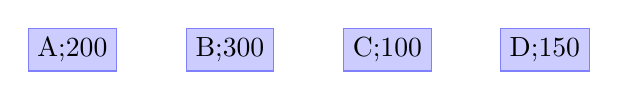
\begin{tikzpicture}
\node at (-4,1) [rectangle,draw=blue!50,fill=blue!20] {A;200};
\node at (-2,1) [rectangle,draw=blue!50,fill=blue!20] {B;300};
\node at ( 0,1) [rectangle,draw=blue!50,fill=blue!20] {C;100};
\node at ( 2,1) [rectangle,draw=blue!50,fill=blue!20] {D;150};
\end{tikzpicture}
\end{center}
}

\only<4>
{
\begin{center}
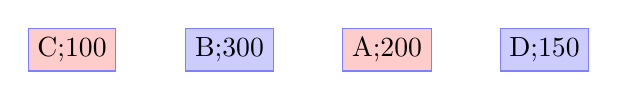
\begin{tikzpicture}
\node at (-4,1) [rectangle,draw=blue!50,fill=red!20] {C;100};
\node at (-2,1) [rectangle,draw=blue!50,fill=blue!20] {B;300};
\node at ( 0,1) [rectangle,draw=blue!50,fill=red!20] {A;200};
\node at ( 2,1) [rectangle,draw=blue!50,fill=blue!20] {D;150};
\end{tikzpicture}
\end{center}
}

\only<5>
{
\begin{center}
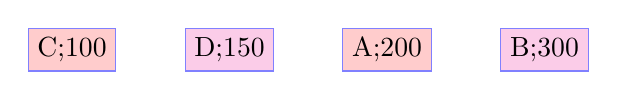
\begin{tikzpicture}
\node at (-4,1) [rectangle,draw=blue!50,fill=red!20] {C;100};
\node at (-2,1) [rectangle,draw=blue!50,fill=magenta!20] {D;150};
\node at ( 0,1) [rectangle,draw=blue!50,fill=red!20] {A;200};
\node at ( 2,1) [rectangle,draw=blue!50,fill=magenta!20] {B;300};
\end{tikzpicture}
\end{center}
}

\only<6>
{
\begin{center}
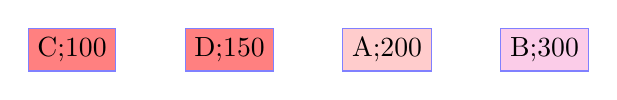
\begin{tikzpicture}
\node at (-4,1) [rectangle,draw=blue!50,fill=red!50] {C;100};
\node at (-2,1) [rectangle,draw=blue!50,fill=red!50] {D;150};
\node at ( 0,1) [rectangle,draw=blue!50,fill=red!20] {A;200};
\node at ( 2,1) [rectangle,draw=blue!50,fill=magenta!20] {B;300};
\end{tikzpicture}
\end{center}
}

\only<7>
{
\begin{center}
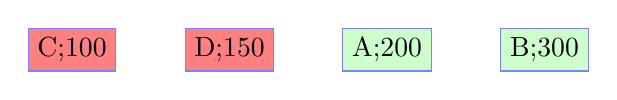
\begin{tikzpicture}
\node at (-4,1) [rectangle,draw=blue!50,fill=red!50] {C;100};
\node at (-2,1) [rectangle,draw=blue!50,fill=red!50] {D;150};
\node at ( 0,1) [rectangle,draw=blue!50,fill=green!20] {A;200};
\node at ( 2,1) [rectangle,draw=blue!50,fill=green!20] {B;300};
\end{tikzpicture}
\end{center}
}

\only<8>
{
\begin{center}
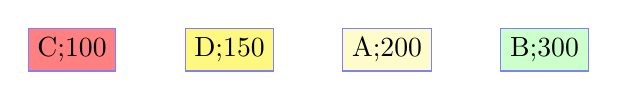
\begin{tikzpicture}
\node at (-4,1) [rectangle,draw=blue!50,fill=red!50] {C;100};
\node at (-2,1) [rectangle,draw=blue!50,fill=yellow!50] {D;150};
\node at ( 0,1) [rectangle,draw=blue!50,fill=yellow!20] {A;200};
\node at ( 2,1) [rectangle,draw=blue!50,fill=green!20] {B;300};
\end{tikzpicture}
\end{center}
}

\end{frame}

\begin{frame}
\frametitle{Security}

Can $\manager$ link the first record in the starting configuration to
its position in the last configuration?

{
\begin{center}
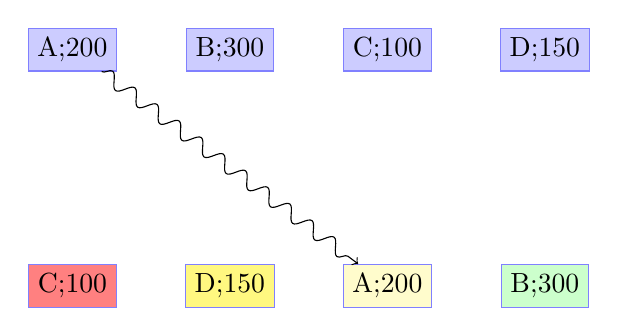
\begin{tikzpicture}
\node at (-4,4) [rectangle,draw=blue!50,fill=blue!20] (as) {A;200};
\node at (-2,4) [rectangle,draw=blue!50,fill=blue!20] (bs) {B;300};
\node at ( 0,4) [rectangle,draw=blue!50,fill=blue!20] (cs) {C;100};
\node at ( 2,4) [rectangle,draw=blue!50,fill=blue!20] (ds) {D;150};

\node at (-4,1) [rectangle,draw=blue!50,fill=red!50]    (cg) {C;100};
\node at (-2,1) [rectangle,draw=blue!50,fill=yellow!50] (dg) {D;150};
\node at ( 0,1) [rectangle,draw=blue!50,fill=yellow!20] (ag) {A;200};
\node at ( 2,1) [rectangle,draw=blue!50,fill=green!20]  (bg) {B;300};
\draw [->,decorate,decoration=snake] (as) -- (ag);
\end{tikzpicture}
\end{center}
}
\end{frame}

\begin{frame}
\frametitle{Two Concepts}
\begin{block}{Indistinguishability of {\em Swap or Not}}
\begin{itemize}
\item  Download, Decrypt, \alert{Swap or Not}, Re-encrypt, Upload
\end{itemize}

\pause
\vskip 1cm
\alert{Chosen-Ciphertext Security}:
Standard notion of security for encryption guarantee that $\manager$ is unable to deduce
if a swap has happened.
\end{block}
\end{frame}

\section{Oblivious Algorithms}
\begin{frame}
\frametitle{Enter Obliviousness}

\begin{definition}[Weak Obliviousness]
An algorithm is {\em \alert{weakly oblivious}} if the {\em access pattern} to data
is the same for all possible inputs of the same length.
\end{definition}
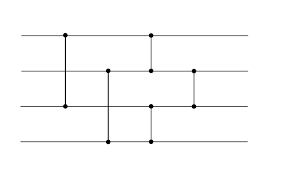
\includegraphics[width=2in]{Images/oramTutorial/sortingNetwork.png}
\vfill
\hfill \tiny{Thanks to Wikipedia for the image}
\end{frame}

\begin{frame}
\frametitle{The adversarial setting}
\begin{center}
\begin{tikzpicture}
[background rectangle/.style={draw=blue!40,fill=brown!20,rounded corners=1ex},
show background rectangle,
local/.style={rectangle,draw=green!50,fill=black!10,thick},
real/.style={rectangle,draw=black!50,fill=black!20,thick,minimum size=7mm},
dumm/.style={rectangle,draw=black!50,fill=magenta!20,thick},
encr/.style={rectangle,draw=red!50,fill=blue!20,thick,minimum size=7mm},
stas/.style={rectangle,draw=black!50,fill=green!20,thick,minimum size=7mm},
esta/.style={rectangle,draw=red!50,fill=green!20,thick,minimum size=7mm}]
\node at (5, 0.0) {};
\node at (-6,-5)  {};
\node at (-6,-2) (leftend) {};
\node at ( 4,-2) (rightend) {};
\node at (-6,-1.7) {{\color{blue} $\manager$}};
\node at (-6,-2.3) {\color{blue} {$\owner$}};
\draw [-,draw=teal,dashed] (leftend) to (rightend);
\node at (-4,0) [encr] (as) {}; \node [above] at (as.north) {1};
\node at (-3,0) [encr] (bs) {}; \node [above] at (bs.north) {2};
\node at (-2,0) [encr] (cs) {}; \node [above] at (cs.north) {3};
\node at (-1,0) [encr] (ds) {}; \node [above] at (ds.north) {4};
\node at ( 0,0) [encr] (es) {}; \node [above] at (es.north) {5};
\node at ( 1,0) [encr] (fs) {}; \node [above] at (fs.north) {6};

\only<2-3>{\node at (-6,-1)[anchor=west]{\textcolor{purple}{Download one or more blocks}};}
\only<3->{\node at (-6,-4) [encr] (xs) {};}
\only<3> {\node at (-5,-4) [encr] (ys) {};}
\only<3>{\draw [->,dotted,draw=brown,thick] (bs.south) to [out=225,in=45] (xs.north);
\draw [->,dotted,draw=brown,thick] (es.south) to [out=225,in=45] (ys.north);}
\only<4> {\node at  (-6,-1)[anchor=west]{\textcolor{purple}{Decrypt one block}};}
\only<4-5>{\node at (-5,-4) [real] (ys) {$B_4$};}
\only<5-6> {\node at  (-6,-1)[anchor=west]{\textcolor{purple}{Re-encrypt}};}
\only<6-8>{\node at (-5,-4) [encr] (ys) {};}
\only<7-> {\node at  (-6,-1)[anchor=west]{\textcolor{purple}{Upload}};}
\only<8>{\draw [->,dotted,draw=brown,thick] (ys.north) to [out=45,in=225] (bs.south);}

\only<3->{\node at (3, 1.0)[anchor=west]{\textcolor{teal}{$\manager$'s {\tt{View}}}};}
\only<3->{\node at (3, 0.0)[anchor=west]{\textcolor{teal}{{\tt{Down(2)}}}};}
\only<3->{\node at (3,-0.4)[anchor=west]{\textcolor{teal}{{\tt{Down(5)}}}};}
\only<8->{\node at (3,-0.8)[anchor=west]{\textcolor{teal}{{\tt{Up(2)}}}};}


\end{tikzpicture}
\end{center}

\end{frame}


\begin{frame}
\frametitle{A new industry}

\begin{block}{Job Opportunities for Algorithmists}
\begin{itemize}
{\color{teal}
\item Re-design all algorithms to be oblivious!
\item Remove all {\em if}s, and {\em while}s
}
\item \alert{Insertion Sort is not oblivious:}
{\color{magenta}
    \begin{itemize}
        \item when the last element of the array is inserted,
            $\manager$ sees where it lands
    \end{itemize}
}
\end{itemize}
\end{block}

\vfill
\pause

\only<2-3>{{\color{blue} Abbiamo abolito la povert\`a}}
\only<3>{\color{red} $\ldots$ per gli algoritmisti}
\only<4>{{\color{green!50} What? Just move on to the next slide and stop talking politics}}

\end{frame}

\begin{frame}
\frametitle{Hiding the Algorithm}

\begin{block}{A new threat}
\begin{itemize}
\item which algorithm is being run \alert{should} also be private information
\end{itemize}

{
\begin{center}
\begin{tikzpicture}
\node at (-4,4) [rectangle,draw=red!50,fill=blue!20] (as) {A;200};
\node at (-2,4) [rectangle,draw=red!50,fill=blue!20] (bs) {B;300};
\node at ( 0,4) [rectangle,draw=red!50,fill=blue!20] (cs) {C;100};
\node at ( 2,4) [rectangle,draw=red!50,fill=blue!20] (ds) {D;150};
\only<2>{
    \node at (-4,2) [rectangle,draw=red!50,fill=blue!20,minimum size=3mm] (d) {};
    \draw [->,dotted,draw=brown,thick] (as.south) to  (d.north);
}
\only<3>{
    \node at (-2,2) [rectangle,draw=red!50,fill=blue!20,minimum size=3mm] (d) {};
    \draw [->,dotted,draw=brown,thick] (bs.south) to  (d.north);
}
\only<4>{
    \node at ( 0,2) [rectangle,draw=red!50,fill=blue!20,minimum size=3mm] (d) {};
    \draw [->,dotted,draw=brown,thick] (cs.south) to  (d.north);
}
\only<5>{
    \node at ( 2,2) [rectangle,draw=red!50,fill=blue!20,minimum size=3mm] (d) {};
    \draw [->,dotted,draw=brown,thick] (ds.south) to  (d.north);
}
\end{tikzpicture}
\end{center}
}
\end{block}
\end{frame}


\begin{frame}[label=GO]
\frametitle{Enter Oblivious RAM \hfill \hyperlink{dp<2>}{\beamergotobutton{Differential Privacy}}}
\begin{block}{ORAM [Goldreich-Ostrovsky]}
\begin{itemize}
\item {\color{blue} $\manager$ stores $n$ blocks of memory.}
\item {\color{blue} Every time $\owner$ wants a block, he asks $\manager$ one or more blocks.}

{\color{olive}
\item Security notion:
\begin{itemize}
\color{olive}
\item For any two block sequences $\color{teal} \mathbb{B}=B_1,\ldots,B_n$ and 
                                    $\color{magenta} \mathbb{C}=C_1,\ldots,C_n$
\item For any two access sequences $\color{teal}   I=(i_1,\ldots,i_l)$ and 
                                   $\color{magenta}J=(j_1,\ldots,j_l)$
\begin{itemize}
\color{olive}
    \item performing accesses $\color{teal}    i_1,\ldots,i_l$ on
                $\color{teal} \mathbb{B}=B_1,\ldots,B_n$;
    \item performing access $\color{magenta} j_1,\ldots,j_l$ on
                $\color{magenta} \mathbb{C}=C_1,\ldots,C_n$
\end{itemize}
\end{itemize}
    generate the same distribution of accesses to the data stored by $\manager$
}
\end{itemize}
\end{block}
\pause
For every predicate $A$
\begin{align*}
\text{\rm Prob}[&\mathtt{view}\leftarrow\mathtt{View}({\color{teal}I,\mathbb{B}}):
    A(\mathtt{view})=1]\\ & \leq e^0\cdot
  \text{\rm Prob}[\mathtt{view}\leftarrow\mathtt{View}({\color{magenta}J,\mathbb{C}}):
    A(\mathtt{view})=1]+{\mathsf{negl}(n)}
\end{align*}
\end{frame}

\begin{frame}
\frametitle{ORAM makes all Algorithms Oblivious}
\begin{block}{Composing ORAM and Non-Oblivious Algorithms}

\begin{itemize}
\item $\owner$ runs the algorithm
\item when a block of memory is requested, $\owner$ retrieves it from $\manager$
using ORAM.
\end{itemize}
\end{block}
\pause
\vfill
\centerline{\alert{Is ORAM possible at all?}}
\end{frame}

\section{An inefficient ORAM}

\begin{frame}[label=zeroConst]
\frametitle{Yes! This is possible!}
\begin{block}{A Trivial ORAM \hfill \hyperlink{recap}{\beamergotobutton{Jump ahead}}}
\begin{itemize}
\item All blocks are uploaded to $\manager$ in encrypted form.
\begin{center}
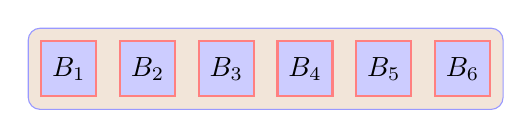
\begin{tikzpicture}
[background rectangle/.style={draw=blue!40,fill=brown!20,rounded corners=1ex},
show background rectangle,
local/.style={rectangle,draw=green!50,fill=black!10,thick},
real/.style={rectangle,draw=black!50,fill=black!20,thick},
dumm/.style={rectangle,draw=black!50,fill=magenta!20,thick},
encr/.style={rectangle,draw=red!50,fill=blue!20,thick,minimum size=7mm},
stas/.style={rectangle,draw=black!50,fill=green!20,thick,minimum size=7mm},
esta/.style={rectangle,draw=red!50,fill=green!20,thick,minimum size=7mm}]
\node at (-4,4) [encr] (as) {$B_1$};
\node at (-3,4) [encr] (bs) {$B_2$};
\node at (-2,4) [encr] (cs) {$B_3$};
\node at (-1,4) [encr] (ds) {$B_4$};
\node at ( 0,4) [encr] (ds) {$B_5$};
\node at ( 1,4) [encr] (ds) {$B_6$};
\end{tikzpicture}
\end{center}
\item Every time $\owner$ needs to access block $B_i$,
    all the blocks are downloaded and all except for $B_i$ are discarded.
\only<2->{
\begin{center}
\begin{tikzpicture}
[background rectangle/.style={draw=blue!40,fill=brown!20,rounded corners=1ex},
show background rectangle,
local/.style={rectangle,draw=green!50,fill=black!10,thick},
real/.style={rectangle,draw=black!50,fill=black!20,thick},
dumm/.style={rectangle,draw=black!50,fill=magenta!20,thick},
encr/.style={rectangle,draw=red!50,fill=blue!20,thick,minimum size=7mm},
stas/.style={rectangle,draw=black!50,fill=green!20,thick,minimum size=7mm},
esta/.style={rectangle,draw=red!50,fill=green!20,thick,minimum size=7mm}]
\node at (-1.5,5) {\textcolor{olive}{Accessing block $B_3$}};
\only<2->{
\node at (-4,4) [encr] (as) {$B_1$};
\node at (-3,4) [encr] (bs) {$B_2$};
\node at (-2,4) [encr] (cs) {$B_3$};
\node at (-1,4) [encr] (ds) {$B_4$};
\node at ( 0,4) [encr] (es) {$B_5$};
\node at ( 1,4) [encr] (fs) {$B_6$};}
\node at (-4,3) [minimum size=5mm](d) {};
\only<3>{
\node at (-4,3) [real] (d) {$B_1$};
\draw [->,dotted,draw=brown,thick] (as.south) to  (d.north);
}
\only<4>{
\node at (-3,3) [real] (d) {$B_2$};
\draw [->,dotted,draw=brown,thick] (bs.south) to  (d.north);
}
\only<5->{\node at (-2,3) [real] (d) {$B_3$};}
\only<5>{
\draw [->,dotted,draw=brown,thick] (cs.south) to  (d.north);
}
\only<6>{
\node at (-1,3) [real] (d) {$B_4$};
\draw [->,dotted,draw=brown,thick] (ds.south) to  (d.north);
}
\only<7>{
\node at ( 0,3) [real] (d) {$B_5$};
\draw [->,dotted,draw=brown,thick] (es.south) to  (d.north);
}
\only<8>{
\node at ( 1,3) [real] (d) {$B_6$};
\draw [->,dotted,draw=brown,thick] (fs.south) to  (d.north);
}
\end{tikzpicture}
\end{center}
}
\end{itemize}
\end{block}

\vfill
\only<9->{{\bf\color{olive} Access pattern independent from the block accessed\par but...}}
\only<10>{\hfill{\bf\color{brown}linear slowdown!!}}
\end{frame}

\section{An insecure ORAM}
\begin{frame}
\frametitle{First try}
\centerline{\alert{\bf Can this be made efficient?}}

\pause
\vskip 1cm 

\begin{block}{First try: Initialization}
\begin{itemize}
\item permute blocks according to permutation $\pi$
    \begin{itemize}
        \item an encryption of $B_i$ is uploaded  in position $\pi(i)$;
    \end{itemize}
\begin{center}
\begin{tikzpicture}
[%%background rectangle/.style={draw=blue!40,fill=brown!20,rounded corners=1ex},
%%show background rectangle,
local/.style={rectangle,draw=green!50,fill=black!10,thick},
real/.style={rectangle,draw=black!50,fill=black!20,thick},
dumm/.style={rectangle,draw=black!50,fill=magenta!20,thick},
encr/.style={rectangle,draw=red!50,fill=blue!20,thick,minimum size=7mm},
stas/.style={rectangle,draw=black!50,fill=green!20,thick,minimum size=7mm},
esta/.style={rectangle,draw=red!50,fill=green!20,thick,minimum size=7mm}]
\only<2>{
\node at (-4,4) [real] (as) {$B_1$};
\node at (-3,4) [real] (bs) {$B_2$};
\node at (-2,4) [real] (cs) {$B_3$};
\node at (-1,4) [real] (ds) {$B_4$};
\node at ( 0,4) [real] (es) {$B_5$};
\node at ( 1,4) [real] (fs) {$B_6$};
}
\only<3->{
\node at (-4,4) [encr] (as) {$B_2$};
\node at (-3,4) [encr] (bs) {$B_4$};
\node at (-2,4) [encr] (cs) {$B_3$};
\node at (-1,4) [encr] (ds) {$B_6$};
\node at ( 0,4) [encr] (es) {$B_1$};
\node at ( 1,4) [encr] (fs) {$B_5$};}
\end{tikzpicture}
\end{center}
\item $\owner$ keeps $\pi$ private;
\end{itemize}
\end{block}
\end{frame}

\begin{frame}
\frametitle{First try}
\centerline{\alert{\bf Can this be made efficient?}}

\begin{block}{First try: Reading block $i$}
\begin{itemize}
    \item ask $\manager$ for block in position $\pi(i)$;
    \item decrypt to obtain $B_i$;
    \item re-encrypt and upload in position $\pi(i)$;
\end{itemize}
\begin{center}
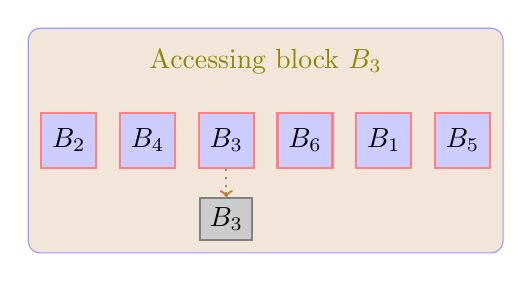
\begin{tikzpicture}
[background rectangle/.style={draw=blue!40,fill=brown!20,rounded corners=1ex},
show background rectangle,
local/.style={rectangle,draw=green!50,fill=black!10,thick},
real/.style={rectangle,draw=black!50,fill=black!20,thick},
dumm/.style={rectangle,draw=black!50,fill=magenta!20,thick},
encr/.style={rectangle,draw=red!50,fill=blue!20,thick,minimum size=7mm},
stas/.style={rectangle,draw=black!50,fill=green!20,thick,minimum size=7mm},
esta/.style={rectangle,draw=red!50,fill=green!20,thick,minimum size=7mm}]
\node at (-1.5,5) {\textcolor{olive}{Accessing block $B_3$}};
\node at (-4,4) [encr] (as) {$B_2$};
\node at (-3,4) [encr] (bs) {$B_4$};
\node at (-2,4) [encr] (cs) {$B_3$};
\node at (-1,4) [encr] (ds) {$B_6$};
\node at ( 0,4) [encr] (es) {$B_1$};
\node at ( 1,4) [encr] (fs) {$B_5$};
\node at (-4,3) [minimum size=5mm](d) {};
\only<2->{
\node at (-2,3) [real] (d) {$B_3$};
\draw [->,dotted,draw=brown,thick] (cs.south) to  (d.north);
}
\end{tikzpicture}
\end{center}
\end{block}
\end{frame}

\begin{frame}
\frametitle{First try: Security}
\begin{block}{Access sequence: $B_1,B_2,B_3$}
\begin{center}
\begin{tikzpicture}
[background rectangle/.style={draw=blue!40,fill=brown!20,rounded corners=1ex},
show background rectangle,
local/.style={rectangle,draw=green!50,fill=black!10,thick},
real/.style={rectangle,draw=black!50,fill=black!20,thick},
dumm/.style={rectangle,draw=black!50,fill=magenta!20,thick},
encr/.style={rectangle,draw=red!50,fill=blue!20,thick,minimum size=7mm},
stas/.style={rectangle,draw=black!50,fill=green!20,thick,minimum size=7mm},
esta/.style={rectangle,draw=red!50,fill=green!20,thick,minimum size=7mm}]
\node at (-6,4) {};
\node at ( 4,4) {};
\node at (-4,4) [encr] (as) {$B_2$}; \node [blue,above] at (as.north) {1};
\node at (-3,4) [encr] (bs) {$B_4$}; \node [blue,above] at (bs.north) {2};
\node at (-2,4) [encr] (cs) {$B_3$}; \node [blue,above] at (cs.north) {3};
\node at (-1,4) [encr] (ds) {$B_6$}; \node [blue,above] at (ds.north) {4};
\node at ( 0,4) [encr] (es) {$B_1$}; \node [blue,above] at (es.north) {5};
\node at ( 1,4) [encr] (fs) {$B_5$}; \node [blue,above] at (fs.north) {6};
\only<1>{\node at (-6,0)[anchor=west]{\textcolor{olive}{Access pattern seen by $\manager: $}};}
\only<2-3>{\node at (-6,0)[anchor=west]{\textcolor{olive}{Access pattern seen by $\manager: 5$}};}
\only<4-5>{\node at (-6,0)[anchor=west]{\textcolor{olive}{Access pattern seen by $\manager: 5,1$}};}
\only<6>{\node at (-6,0)[anchor=west]{\textcolor{olive}{Access pattern seen by $\manager: 5,1,3$}};}
\only<7>{\node at (-6,0)[anchor=west]{\textcolor{olive}{Access pattern seen by $\manager: x,y,z$}};}

\only<1-2>{\node at (-4.5,5){\textcolor{olive}{Accessing block $B_1$}};}
\only<2>{
\node at ( 0,3) [real] (d1) {$B_1$};
\draw [->,dotted,draw=brown,thick] (es.south) to  (d1.north);
}

\only<3-4>{\node at (-4.5,5){\textcolor{olive}{Accessing block $B_2$}};}
\only<4>{
\node at (-4,3) [real] (d2) {$B_2$};
\draw [->,dotted,draw=brown,thick] (as.south) to  (d2.north);
}

\only<5-6>{\node at (-4.5,5){\textcolor{olive}{Accessing block $B_3$}};}
\only<6>{
\node at (-2,3) [real] (d3) {$B_3$};
\draw [->,dotted,draw=brown,thick] (cs.south) to  (d3.north);
}
\end{tikzpicture}
\end{center}
\end{block}
\end{frame}

\begin{frame}
\frametitle{First try: Security}
\begin{block}{Access sequence: $B_1,B_2,B_1$}
\begin{center}
\begin{tikzpicture}
[background rectangle/.style={draw=blue!40,fill=brown!20,rounded corners=1ex},
show background rectangle,
local/.style={rectangle,draw=green!50,fill=black!10,thick},
real/.style={rectangle,draw=black!50,fill=black!20,thick},
dumm/.style={rectangle,draw=black!50,fill=magenta!20,thick},
encr/.style={rectangle,draw=red!50,fill=blue!20,thick,minimum size=7mm},
stas/.style={rectangle,draw=black!50,fill=green!20,thick,minimum size=7mm},
esta/.style={rectangle,draw=red!50,fill=green!20,thick,minimum size=7mm}]
\node at (-6,4) {};
\node at ( 4,4) {};
\node at (-4,4) [encr] (as) {$B_2$}; \node [blue,above] at (as.north) {1};
\node at (-3,4) [encr] (bs) {$B_4$}; \node [blue,above] at (bs.north) {2};
\node at (-2,4) [encr] (cs) {$B_3$}; \node [blue,above] at (cs.north) {3};
\node at (-1,4) [encr] (ds) {$B_6$}; \node [blue,above] at (ds.north) {4};
\node at ( 0,4) [encr] (es) {$B_1$}; \node [blue,above] at (es.north) {5};
\node at ( 1,4) [encr] (fs) {$B_5$}; \node [blue,above] at (fs.north) {6};
\only<1>{\node at (-6,0)[anchor=west]{\textcolor{olive}{Access pattern seen by $\manager: $}};}
\only<2-3>{\node at (-6,0)[anchor=west]{\textcolor{olive}{Access pattern seen by $\manager: 5$}};}
\only<4-5>{\node at (-6,0)[anchor=west]{\textcolor{olive}{Access pattern seen by $\manager: 5,1$}};}
\only<6>{\node at (-6,0)[anchor=west]{\textcolor{olive}{Access pattern seen by $\manager: 5,1,5$}};}
\only<7>{\node at (-6,0)[anchor=west]{\textcolor{olive}{Access pattern seen by $\manager: x,y,x$}};}

\only<1-2>{\node at (-4.5,5){\textcolor{olive}{Accessing block $B_1$}};}
\only<2>{
\node at ( 0,3) [real] (d1) {$B_1$};
\draw [->,dotted,draw=brown,thick] (es.south) to  (d1.north);
}

\only<3-4>{\node at (-4.5,5){\textcolor{olive}{Accessing block $B_2$}};}
\only<4>{
\node at (-4,3) [real] (d2) {$B_2$};
\draw [->,dotted,draw=brown,thick] (as.south) to  (d2.north);
}

\only<5-6>{\node at (-4.5,5){\textcolor{olive}{Accessing block $B_1$}};}
\only<6>{
\node at ( 0,3) [real] (d3) {$B_1$};
\draw [->,dotted,draw=brown,thick] (es.south) to  (d3.north);
}
\end{tikzpicture}
\end{center}
\end{block}
\end{frame}

\begin{frame}
\frametitle{Oblivious RAM}

\begin{block}{Obliviousness}
For any two {\em access sequences}
$O_1=(i_1^1,\ldots,i_l^1)$ 
$O_2=(i_1^2,\ldots,i_l^2)$ of the same length,
the distribution of the positions requested by $\owner$ to $\manager$ is the same.
\end{block}
\pause

\vfill

\begin{block}{Oblivious for Non-repeating sequences}
\begin{itemize}
\item $k_1\ne k_2$ implies $i_{k_1}^1\ne i_{k_2}^1$ and $i_{k_1}^2\ne i_{k_2}^1$;
\item $\manager$ sees requests for $l$ different randomly chosen blocks
both for $O_1$ and for $O_2$.
\end{itemize}
\end{block}
\end{frame}

\begin{frame}
\frametitle{Repetition Pattern is leaked}

\begin{block}{Repetition Pattern}

If the same block is requested twice by $\owner$ 
then $\manager$ sees the same position accessed twice.

\vskip 1cm 
\begin{tabular}{lrrrrrrrrrrr}
{\color{blue} Block}   & 3  & {\color{red} 4} & 7 & {\color{brown} 8} & {\color{red} 4} & 2 & {\color{red} 4}  & 10 & 12 & {\color{brown} 8} & 6 \\
\\
{\color{magenta} Position} & 12 & {\color{red} 2} & 9 & {\color{brown} 3} & {\color{red} 2} & 6 & {\color{red} 2}  & 10 & 1  & {\color{brown} 3} & 5\\
\end{tabular}

\end{block}
\end{frame}

\section{A first secure ORAM}
\begin{frame}
\frametitle{Hiding the Repetition Pattern}
\begin{block}{Initialization for $N$ blocks}
\begin{enumerate}
\item {\color{blue} $N$ {\em real} blocks $B_1,\ldots,B_N$};
\item create {\color{magenta}$M$ {\em dummy} blocks $B_{N+1},\ldots,B_{N+M}$};
\item create {\color{teal}$M$ {\em stash} blocks $S_1,\ldots,S_M$}
    initialized to $0$;
\item pick a random permutation $\pi$ over $[N+M]$;
\item permute {\color{blue} \em real} and {\color{magenta} \em dummy} blocks according to permutation $\pi$
    \begin{itemize}
        \item an {\color{red} encryption of $B_i$} is uploaded  in position $\pi(i)$;
    \end{itemize}
\item upload all {\color{teal} stash blocks} in encrypted form;
\item initialize {\color{teal} $\nxt=1,\cnt=1$};
\item $\pi$ is kept private;
\end{enumerate}
\end{block}
\end{frame}

\begin{frame}
\frametitle{Initial Configuration}
\begin{center}
\begin{tikzpicture}
[background rectangle/.style={draw=blue!40,fill=brown!20,rounded corners=1ex},
show background rectangle,
local/.style={rectangle,draw=green!50,fill=black!10,thick},
real/.style={rectangle,draw=black!50,fill=black!20,thick},
dumm/.style={rectangle,draw=black!50,fill=magenta!20,thick},
encr/.style={rectangle,draw=red!50,fill=blue!20,thick,minimum size=7mm},
stas/.style={rectangle,draw=black!50,fill=green!20,thick,minimum size=7mm},
esta/.style={rectangle,draw=red!50,fill=green!20,thick,minimum size=7mm}]

\only<1-2>{\node at (-3,-5)[rectangle,draw=green!50,minimum size=1mm]{};}

\only<1-3>{
\node at (-5,0)    [real] (uno)   {$B_1$};
\node at (-4.2,0)  [real] (due)   {$B_2$};
\node at (-3.5,0)                 {$\ldots$};
\node at (-3.0,0)                 {$\ldots$};
\node at (-2.5,0)  [real] (enne)  {$B_N$};
\node at (-1.3,0)  [dumm] (d1)    {$B_{_{N+1}}$};
\node at (-0.2,0)  [dumm] (d2)    {$B_{_{N+2}}$};
\node at (0.6,0)                  {$\ldots$};
\node at (1.1,0)                  {$\ldots$};
\node at (1.6,0)   [dumm] (dm)    {$B_{_{N+M}}$};
\node at (-3.5,.9) [real] (realb) {\textcolor{gray}{Real Blocks}};
\node at (-0.0,.9) [dumm] (dummb) {\textcolor{magenta}{Dummy Blocks}};
\node at ( 4.4,.9) [stas] (stasb) {\textcolor{green}{Stash}};
\node at (3.2,0)   [stas] (s1)    {$0$};
\node at (4.0,0)   [stas] (s2)    {$0$};
\node at (4.65,0)                 {$\ldots$};
\node at (5.3,0)   [stas] (sm)    {$0$};
\draw [->,dotted,draw=red,thick] (realb.west) to  [out=140,in=120]  (uno.west);
\draw [->,dotted,draw=red,thick] (realb.south) to  [out=220,in=45]  (due.north);
\draw [->,dotted,draw=red,thick] (realb.south) to  [out=315,in=135] (enne.north);
\draw [->,dotted,draw=red,thick] (dummb.west) to  [out=140,in=120]  (d1.west);
\draw [->,dotted,draw=red,thick] (dummb.south) to  [out=220,in=45]  (d2.north);
\draw [->,dotted,draw=red,thick] (dummb.south) to  [out=315,in=135] (dm.north);
}


\only<2->{
\node at (-5,-2)    [encr] (unoe)  {};
\node at (-4.2,-2)  [encr] (duee)  {};
\node at (-3.4,-2)  [encr] (tree)  {};
\node at (-2.75,-2)                {$\ldots$};
\node at (-2.1,-2)  [encr] (ennee) {};
\node at (-1.45,-2)                {$\ldots$};
\node at (-0.8,-2)  [encr] (d1e)   {};
\node at ( 0.0,-2)  [encr] (d2e)   {};
\node at ( 0.65,-2)                {$\ldots$};
\node at (1.3,-2)   [encr] (dme)   {};
\node at (3.2,-2)   [esta] (se1)   {$0$};
\node at (4.0,-2)   [esta] (se2)   {$0$};
\node at (4.65,-2)                 {$\ldots$};
\node at (5.3,-2)   [esta] (sem)   {$0$};
}


\only<2-3>{
\node at (-5,-3)           (unop)   {\textcolor{magenta}{\small$\pi(N)$}};
\draw [->,dotted,draw=red,thick] (unop.west) to [out=180,in=180] (unoe.west);
\node at (0,-3)           (ennep)   {\textcolor{magenta}{\small$\pi(2)$}};
\draw [->,dotted,draw=red,thick] (ennep.west) to [out=180,in=270] (ennee.south);
\node at (1.3,-3)           (emmep)   {\textcolor{magenta}{\small$\pi(1)$}};
\draw [->,dotted,draw=red,thick] (emmep.east) to [out=0,in=0] (dme.east);

\draw [->,draw=brown,thick] (uno.south) to [out=270,in=90] (dme.north);
\draw [->,draw=brown,thick] (due.south) to [out=270,in=90] (ennee.north);
\draw [->,draw=brown,thick] (enne.south)to [out=270,in=90] (unoe.north);
\draw [->,draw=brown,thick] (d1.south)  to [out=270,in=90] (duee.north);
\draw [->,draw=brown,thick] (d2.south)  to [out=270,in=90] (d2e.north);
\draw [->,draw=brown,thick] (dm.south)  to [out=270,in=90] (d1e.north);
\draw [->,draw=brown,thick] (s1.south)  to                 (se1.north);
\draw [->,draw=brown,thick] (s2.south)  to                 (se2.north);
\draw [->,draw=brown,thick] (sm.south)  to                 (sem.north);
}
\only<3->{
\node at (-5.8,-1.4)[rectangle,anchor=north west,draw=red,dashed,minimum height=12mm,minimum width=11.8cm] (server) {};
}
\only<3>{
\node at (-2,-3.65) [encr] {\textcolor{gray}{$N+M$ Encrypted Blocks}};
\node at ( 4,-3.65) [esta] {\textcolor{gray}{$M$ Encrypted Stash}};
}
\only<4->{
\node at (-4.5,-5) [local] (cnt) {\textcolor{black!40}{${\mathsf{cnt}}=1$}};
\node at (-2.5,-5) [local] (nxt) {\textcolor{black!40}{${\mathsf{nxt}}=1$}};
\node at (-0.5,-5) [local] (pi)  {\textcolor{black!40}{${\mathsf{\pi}}$}};
\node at (3,-5) [local] (loc) {\textcolor{teal}{Local to $\owner$}};
\node at (3,-4) [encr] (serv1) {\textcolor{gray}{$\manager$'s storage}};
\node at (-5.6,-4.4)[rectangle,anchor=north west,draw=red,dashed,minimum height=12mm,minimum width=5.8cm] (client) {};
\draw [->,draw=brown,thick] (serv1.north)  to  [out=90,in=270] (server.south);
\draw [->,draw=brown,thick] (loc.west)  to  [out=180,in=0] (client.east);
%%\draw [->,dotted,draw=red,thick] (loc.west)  to  [out=180,in=0] (cnt.east);
%%\draw [->,dotted,draw=red,thick] (loc.east)  to  [out=0,in=180] (pi.west);
%%\draw [->,dotted,draw=red,thick] (loc.north) to  [out=90,in=300] (nxt.south);
}

\end{tikzpicture}
\end{center}
\end{frame}

\begin{frame}
\begin{block}{Reading Block $B_i$}
\begin{enumerate}
    \item download and decrypt all {\color{teal} $M$ blocks in the Stash};
    \item if $B_i$ is found in the {\color{teal} Stash} then
    \begin{itemize}
    \item {\color{magenta} download dummy block $\pi(N+\cnt)$};
    \item {\color{teal} set $\cnt=\cnt+1$};
    \end{itemize}
    \item[] else
    \begin{itemize}
    \item download {\color{red} encrypted real block in position $\pi(i)$};
    \item decrypt and obtain {\color{blue} real block $B_i$};
    \item set {\color{teal} next available Stash block $S_\nxt=B_i$};
    \item {\color{teal} set $\nxt=\nxt+1$};
    \end{itemize}
    \item re-encrypt and upload {\color{teal} all blocks in the Stash};
\end{enumerate}
\end{block}

\end{frame}

\begin{frame}
\frametitle{Reading Block $B_1$}
{\color{brown} Download and decrypt all blocks from Stash}
\begin{center}
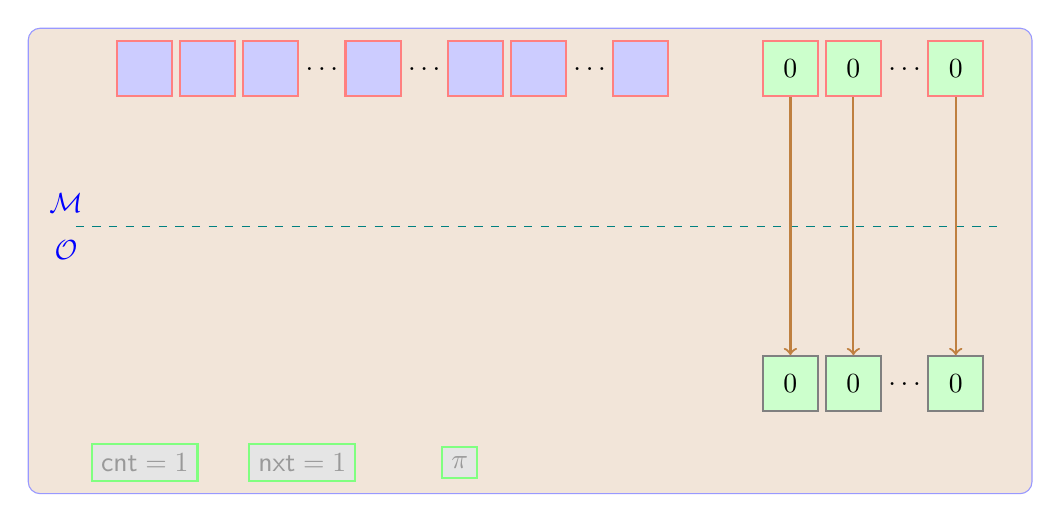
\begin{tikzpicture}
[background rectangle/.style={draw=blue!40,fill=brown!20,rounded corners=1ex},
show background rectangle,
local/.style={rectangle,draw=green!50,fill=black!10,thick},
real/.style={rectangle,draw=black!50,fill=black!20,thick},
dumm/.style={rectangle,draw=black!50,fill=magenta!20,thick},
encr/.style={rectangle,draw=red!50,fill=blue!20,thick,minimum size=7mm},
stas/.style={rectangle,draw=black!50,fill=green!20,thick,minimum size=7mm},
esta/.style={rectangle,draw=red!50,fill=green!20,thick,minimum size=7mm}]
\node at (-6,-4) (leftend) {};
\node at ( 6,-4) (rightend) {};
\node at (-6,-3.7) {{\color{blue} $\manager$}};
\node at (-6,-4.3) {\color{blue} {$\owner$}};
\draw [-,draw=teal,dashed] (leftend) to (rightend);

\node at (-5,-2)    [encr] (unoe)   {};
\node at (-4.2,-2)  [encr] (duee)   {};
\node at (-3.4,-2)  [encr] (tree)   {};
\node at (-2.75,-2)                 {$\ldots$};
\node at (-2.1,-2)  [encr] (ennee) {};
\node at (-1.45,-2)                 {$\ldots$};
\node at (-0.8,-2)  [encr] (d1e)   {};
\node at ( 0.0,-2)  [encr] (d2e)   {};
\node at ( 0.65,-2)                 {$\ldots$};
\node at (1.3,-2)   [encr] (dme)   {};
\node at (3.2,-2)   [esta] (se1)   {$0$};
\node at (4.0,-2)   [esta] (se2)   {$0$};
\node at (4.65,-2)                 {$\ldots$};
\node at (5.3,-2)   [esta] (sem)   {$0$};

\node at (3.2,-6)   [stas] (se1d)   {$0$};
\node at (4.0,-6)   [stas] (se2d)   {$0$};
\node at (4.65,-6)                 {$\ldots$};
\node at (5.3,-6)   [stas] (semd)   {$0$};
\draw [->,draw=brown,thick] (se1.south) to (se1d.north);
\draw [->,draw=brown,thick] (se2.south) to (se2d.north);
\draw [->,draw=brown,thick] (sem.south) to (semd.north);
\node at (-5,-7) [local] (cnt) {\textcolor{black!40}{${\mathsf{cnt}}=1$}};
\node at (-3,-7) [local] (nxt) {\textcolor{black!40}{${\mathsf{nxt}}=1$}};
\node at (-1,-7) [local] (pi)  {\textcolor{black!40}{${\mathsf{\pi}}$}};
\end{tikzpicture}
\end{center}

\pause

\vfill {\color{blue} $B_1$ is not found in the stash}
\end{frame}

\begin{frame}
\frametitle{Reading Block $B_1$}
{\color{brown} Download block in position $\pi(1)$}
\begin{center}
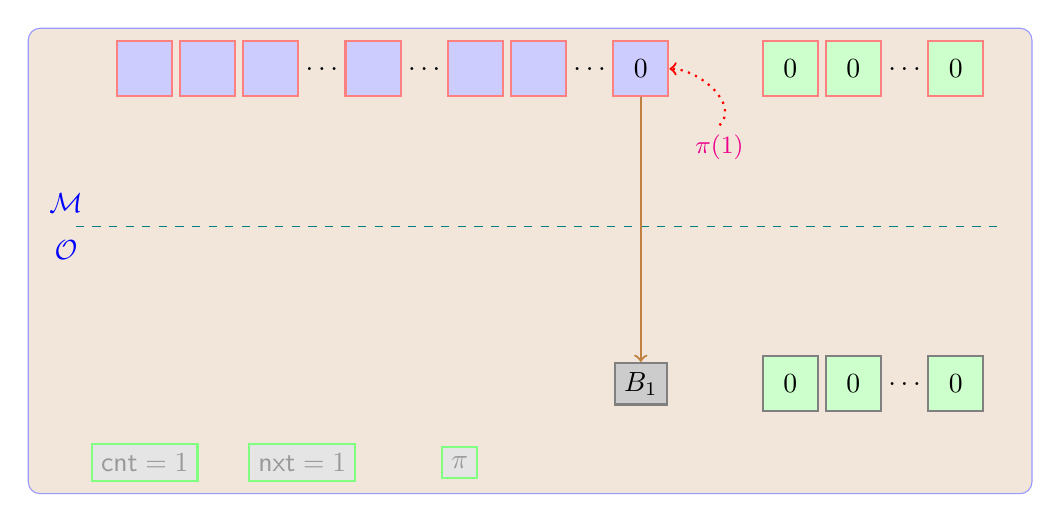
\begin{tikzpicture}
[background rectangle/.style={draw=blue!40,fill=brown!20,rounded corners=1ex},
show background rectangle,
local/.style={rectangle,draw=green!50,fill=black!10,thick},
real/.style={rectangle,draw=black!50,fill=black!20,thick},
dumm/.style={rectangle,draw=black!50,fill=magenta!20,thick},
encr/.style={rectangle,draw=red!50,fill=blue!20,thick,minimum size=7mm},
stas/.style={rectangle,draw=black!50,fill=green!20,thick,minimum size=7mm},
esta/.style={rectangle,draw=red!50,fill=green!20,thick,minimum size=7mm}]

\node at (-6,-4) (leftend) {};
\node at ( 6,-4) (rightend) {};
\node at (-6,-3.7) {{\color{blue} $\manager$}};
\node at (-6,-4.3) {\color{blue} {$\owner$}};
\draw [-,draw=teal,dashed] (leftend) to (rightend);
\node at (-5,-2)    [encr] (unoe)   {};
\node at (-4.2,-2)  [encr] (duee)   {};
\node at (-3.4,-2)  [encr] (tree)   {};
\node at (-2.75,-2)                 {$\ldots$};
\node at (-2.1,-2)  [encr] (ennee) {};
\node at (-1.45,-2)                 {$\ldots$};
\node at (-0.8,-2)  [encr] (d1e)   {};
\node at ( 0.0,-2)  [encr] (d2e)   {};
\node at ( 0.65,-2)                 {$\ldots$};
\node at (1.3,-2)   [encr] (dme)   {$0$};
\node at (3.2,-2)   [esta] (se1)   {$0$};
\node at (4.0,-2)   [esta] (se2)   {$0$};
\node at (4.65,-2)                 {$\ldots$};
\node at (5.3,-2)   [esta] (sem)   {$0$};

\node at (3.2,-6)   [stas] (se1d)   {$0$};
\node at (4.0,-6)   [stas] (se2d)   {$0$};
\node at (4.65,-6)                 {$\ldots$};
\node at (5.3,-6)   [stas] (semd)   {$0$};

\node at (2.3,-3)           (emmep)   {\textcolor{magenta}{\small$\pi(1)$}};
\draw [->,dotted,draw=red,thick] (emmep.north) to [out=45,in=0] (dme.east);

\node at (-5,-7) [local] (cnt) {\textcolor{black!40}{${\mathsf{cnt}}=1$}};
\node at (-3,-7) [local] (nxt) {\textcolor{black!40}{${\mathsf{nxt}}=1$}};
\node at (-1,-7) [local] (pi)  {\textcolor{black!40}{${\mathsf{\pi}}$}};
\node at (1.3,-6)   [real] (dmed)   {$B_1$};
\draw [->,draw=brown,thick] (dme.south) to (dmed.north);
\end{tikzpicture}
\end{center}
\pause
{\color{blue} Decrypt and obtain $B_1$}
\end{frame}

\begin{frame}
\frametitle{Reading Block $B_1$}
{\color{brown} Copy $B_1$ in the Stash at position $\nxt$ }
\begin{center}
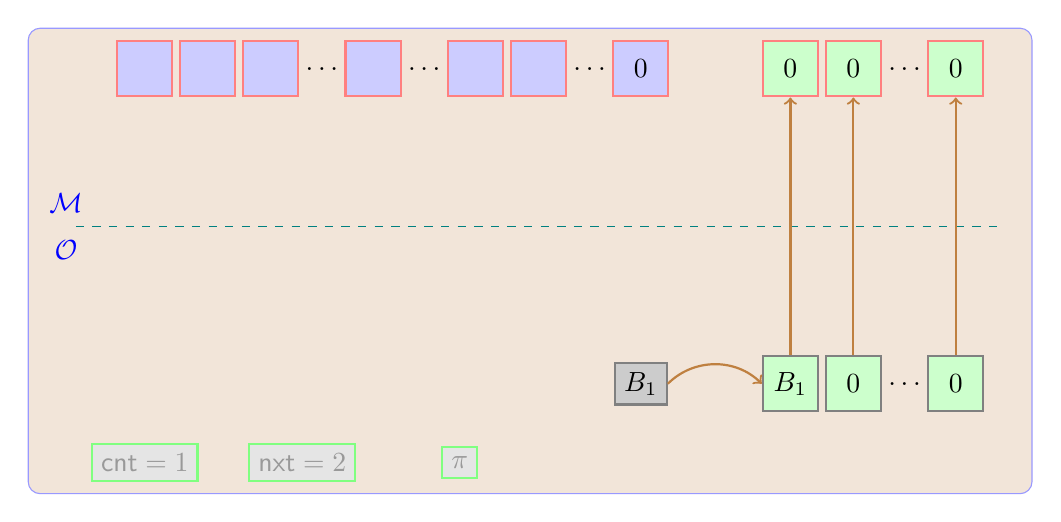
\begin{tikzpicture}
[background rectangle/.style={draw=blue!40,fill=brown!20,rounded corners=1ex},
show background rectangle,
local/.style={rectangle,draw=green!50,fill=black!10,thick},
real/.style={rectangle,draw=black!50,fill=black!20,thick},
dumm/.style={rectangle,draw=black!50,fill=magenta!20,thick},
encr/.style={rectangle,draw=red!50,fill=blue!20,thick,minimum size=7mm},
stas/.style={rectangle,draw=black!50,fill=green!20,thick,minimum size=7mm},
esta/.style={rectangle,draw=red!50,fill=green!20,thick,minimum size=7mm}]

\node at (-6,-4) (leftend) {};
\node at ( 6,-4) (rightend) {};
\node at (-6,-3.7) {{\color{blue} $\manager$}};
\node at (-6,-4.3) {\color{blue} {$\owner$}};
\draw [-,draw=teal,dashed] (leftend) to (rightend);
\node at (-5,-2)    [encr] (unoe)   {};
\node at (-4.2,-2)  [encr] (duee)   {};
\node at (-3.4,-2)  [encr] (tree)   {};
\node at (-2.75,-2)                 {$\ldots$};
\node at (-2.1,-2)  [encr] (ennee) {};
\node at (-1.45,-2)                 {$\ldots$};
\node at (-0.8,-2)  [encr] (d1e)   {};
\node at ( 0.0,-2)  [encr] (d2e)   {};
\node at ( 0.65,-2)                 {$\ldots$};
\node at (1.3,-2)   [encr] (dme)   {$0$};
\node at (3.2,-2)   [esta] (se1)   {$0$};
\node at (4.0,-2)   [esta] (se2)   {$0$};
\node at (4.65,-2)                 {$\ldots$};
\node at (5.3,-2)   [esta] (sem)   {$0$};

\node at (3.2,-6)   [stas] (se1d)   {$B_1$};
\node at (4.0,-6)   [stas] (se2d)   {$0$};
\node at (4.65,-6)                 {$\ldots$};
\node at (5.3,-6)   [stas] (semd)   {$0$};




\node at (-5,-7) [local] (cnt) {\textcolor{black!40}{${\mathsf{cnt}}=1$}};
\node at (-3,-7) [local] (nxt) {\textcolor{black!40}{${\mathsf{nxt}}=2$}};
\node at (-1,-7) [local] (pi)  {\textcolor{black!40}{${\mathsf{\pi}}$}};
\node at (1.3,-6)   [real] (dmed)   {$B_1$};
\draw [->,draw=brown,thick] (dmed.east) to [out=45,in=135] (se1d.west);
\only<2>{
\draw [<-,draw=brown,thick] (se1.south) to (se1d.north);
\draw [<-,draw=brown,thick] (se2.south) to (se2d.north);
\draw [<-,draw=brown,thick] (sem.south) to (semd.north);
}
\end{tikzpicture}
\end{center}
\pause
{\color{blue} Encrypt and Upload the Stash}
\end{frame}

\begin{frame}
\frametitle{Reading Block $B_2$}
{\color{brown} Download and decrypt all blocks from Stash}
\begin{center}
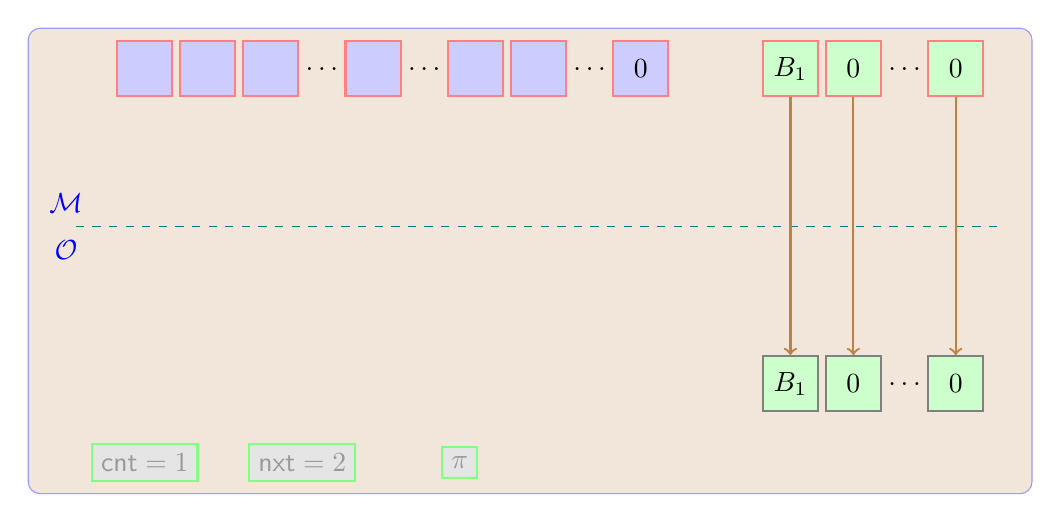
\begin{tikzpicture}
[background rectangle/.style={draw=blue!40,fill=brown!20,rounded corners=1ex},
show background rectangle,
local/.style={rectangle,draw=green!50,fill=black!10,thick},
real/.style={rectangle,draw=black!50,fill=black!20,thick},
dumm/.style={rectangle,draw=black!50,fill=magenta!20,thick},
encr/.style={rectangle,draw=red!50,fill=blue!20,thick,minimum size=7mm},
stas/.style={rectangle,draw=black!50,fill=green!20,thick,minimum size=7mm},
esta/.style={rectangle,draw=red!50,fill=green!20,thick,minimum size=7mm}]

\node at (-6,-4) (leftend) {};
\node at ( 6,-4) (rightend) {};
\node at (-6,-3.7) {{\color{blue} $\manager$}};
\node at (-6,-4.3) {\color{blue} {$\owner$}};
\draw [-,draw=teal,dashed] (leftend) to (rightend);
\node at (-5,-2)    [encr] (unoe)   {};
\node at (-4.2,-2)  [encr] (duee)   {};
\node at (-3.4,-2)  [encr] (tree)   {};
\node at (-2.75,-2)                 {$\ldots$};
\node at (-2.1,-2)  [encr] (ennee) {};
\node at (-1.45,-2)                 {$\ldots$};
\node at (-0.8,-2)  [encr] (d1e)   {};
\node at ( 0.0,-2)  [encr] (d2e)   {};
\node at ( 0.65,-2)                 {$\ldots$};
\node at (1.3,-2)   [encr] (dme)   {$0$};
\node at (3.2,-2)   [esta] (se1)   {$B_1$};
\node at (4.0,-2)   [esta] (se2)   {$0$};
\node at (4.65,-2)                 {$\ldots$};
\node at (5.3,-2)   [esta] (sem)   {$0$};

\node at (3.2,-6)   [stas] (se1d)   {$B_1$};
\node at (4.0,-6)   [stas] (se2d)   {$0$};
\node at (4.65,-6)                 {$\ldots$};
\node at (5.3,-6)   [stas] (semd)   {$0$};
\draw [->,draw=brown,thick] (se1.south) to (se1d.north);
\draw [->,draw=brown,thick] (se2.south) to (se2d.north);
\draw [->,draw=brown,thick] (sem.south) to (semd.north);



\node at (-5,-7) [local] (cnt) {\textcolor{black!40}{${\mathsf{cnt}}=1$}};
\node at (-3,-7) [local] (nxt) {\textcolor{black!40}{${\mathsf{nxt}}=2$}};
\node at (-1,-7) [local] (pi)  {\textcolor{black!40}{${\mathsf{\pi}}$}};
\end{tikzpicture}
\end{center}
\pause {\color{blue} $B_2$ is not found in the Stash}
\end{frame}

\begin{frame}
\frametitle{Reading Block $B_2$}
{\color{brown} Download block in position $\pi(2)$}
\begin{center}
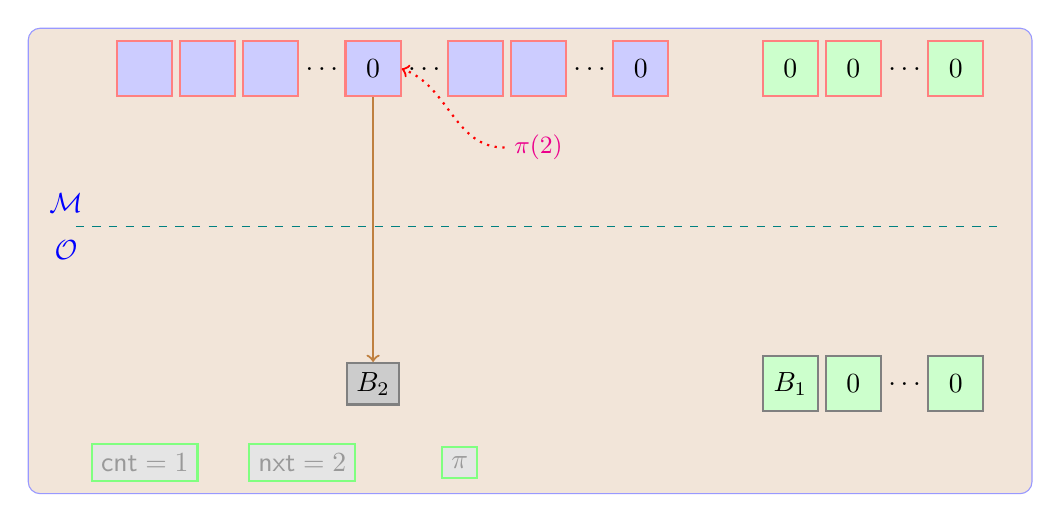
\begin{tikzpicture}
[background rectangle/.style={draw=blue!40,fill=brown!20,rounded corners=1ex},
show background rectangle,
local/.style={rectangle,draw=green!50,fill=black!10,thick},
real/.style={rectangle,draw=black!50,fill=black!20,thick},
dumm/.style={rectangle,draw=black!50,fill=magenta!20,thick},
encr/.style={rectangle,draw=red!50,fill=blue!20,thick,minimum size=7mm},
stas/.style={rectangle,draw=black!50,fill=green!20,thick,minimum size=7mm},
esta/.style={rectangle,draw=red!50,fill=green!20,thick,minimum size=7mm}]

\node at (-6,-4) (leftend) {};
\node at ( 6,-4) (rightend) {};
\node at (-6,-3.7) {{\color{blue} $\manager$}};
\node at (-6,-4.3) {\color{blue} {$\owner$}};
\draw [-,draw=teal,dashed] (leftend) to (rightend);
\node at (-5,-2)    [encr] (unoe)   {};
\node at (-4.2,-2)  [encr] (duee)   {};
\node at (-3.4,-2)  [encr] (tree)   {};
\node at (-2.75,-2)                 {$\ldots$};
\node at (-2.1,-2)  [encr] (ennee) {$0$};
\node at (-1.45,-2)                 {$\ldots$};
\node at (-0.8,-2)  [encr] (d1e)   {};
\node at ( 0.0,-2)  [encr] (d2e)   {};
\node at ( 0.65,-2)                 {$\ldots$};
\node at (1.3,-2)   [encr] (dme)   {$0$};
\node at (3.2,-2)   [esta] (se1)   {$0$};
\node at (4.0,-2)   [esta] (se2)   {$0$};
\node at (4.65,-2)                 {$\ldots$};
\node at (5.3,-2)   [esta] (sem)   {$0$};

\node at (3.2,-6)   [stas] (se1d)   {$B_1$};
\node at (4.0,-6)   [stas] (se2d)   {$0$};
\node at (4.65,-6)                 {$\ldots$};
\node at (5.3,-6)   [stas] (semd)   {$0$};
\node at (-5,-7) [local] (cnt) {\textcolor{black!40}{${\mathsf{cnt}}=1$}};
\node at (-3,-7) [local] (nxt) {\textcolor{black!40}{${\mathsf{nxt}}=2$}};
\node at (-1,-7) [local] (pi)  {\textcolor{black!40}{${\mathsf{\pi}}$}};
\node at (0,-3)           (ennep)   {\textcolor{magenta}{\small$\pi(2)$}};
\draw [->,dotted,draw=red,thick] (ennep.west) to [out=180,in=340] (ennee.east);
\node at (-2.1,-6)   [real] (dmed)   {$B_2$};
\draw [->,draw=brown,thick] (ennee.south) to (dmed.north);
\end{tikzpicture}
\end{center}
\pause
{\color{blue} Decrypt and obtain $B_2$}
\end{frame}

\begin{frame}
\frametitle{Reading Block $B_2$}
{\color{brown} Copy $B_2$ in the Stash at position $\nxt$}
\begin{center}
\begin{tikzpicture}
[background rectangle/.style={draw=blue!40,fill=brown!20,rounded corners=1ex},
show background rectangle,
local/.style={rectangle,draw=green!50,fill=black!10,thick},
real/.style={rectangle,draw=black!50,fill=black!20,thick},
dumm/.style={rectangle,draw=black!50,fill=magenta!20,thick},
encr/.style={rectangle,draw=red!50,fill=blue!20,thick,minimum size=7mm},
stas/.style={rectangle,draw=black!50,fill=green!20,thick,minimum size=7mm},
esta/.style={rectangle,draw=red!50,fill=green!20,thick,minimum size=7mm}]

\node at (-6,-4) (leftend) {};
\node at ( 6,-4) (rightend) {};
\node at (-6,-3.7) {{\color{blue} $\manager$}};
\node at (-6,-4.3) {\color{blue} {$\owner$}};
\draw [-,draw=teal,dashed] (leftend) to (rightend);
\node at (-5,-2)    [encr] (unoe)   {};
\node at (-4.2,-2)  [encr] (duee)   {};
\node at (-3.4,-2)  [encr] (tree)   {};
\node at (-2.75,-2)                 {$\ldots$};
\node at (-2.1,-2)  [encr] (ennee) {$0$};
\node at (-1.45,-2)                 {$\ldots$};
\node at (-0.8,-2)  [encr] (d1e)   {};
\node at ( 0.0,-2)  [encr] (d2e)   {};
\node at ( 0.65,-2)                 {$\ldots$};
\node at (1.3,-2)   [encr] (dme)   {$0$};
\node at (3.2,-2)   [esta] (se1)   {$0$};
\node at (4.0,-2)   [esta] (se2)   {$0$};
\node at (4.65,-2)                 {$\ldots$};
\node at (5.3,-2)   [esta] (sem)   {$0$};

\node at (3.2,-6)   [stas] (se1d)   {$B_1$};
\node at (4.0,-6)   [stas] (se2d)   {$B_2$};
\node at (4.65,-6)                 {$\ldots$};
\node at (5.3,-6)   [stas] (semd)   {$0$};
\node at (-5,-7) [local] (cnt) {\textcolor{black!40}{${\mathsf{cnt}}=1$}};
\node at (-3,-7) [local] (nxt) {\textcolor{black!40}{${\mathsf{nxt}}=3$}};
\node at (-1,-7) [local] (pi)  {\textcolor{black!40}{${\mathsf{\pi}}$}};
\only<1>{\node at (-2.1,-6)   [real] (dmed)   {$B_2$};
\draw [->,draw=brown,thick] (dmed.north) to [out=45,in=135](se2d.north);}
\only<2>{
\draw [<-,draw=brown,thick] (se1.south) to (se1d.north);
\draw [<-,draw=brown,thick] (se2.south) to (se2d.north);
\draw [<-,draw=brown,thick] (sem.south) to (semd.north);
}
\end{tikzpicture}
\end{center}
\pause
{\color{blue} Encrypt and Upload the Stash}
\end{frame}

\begin{frame}
\frametitle{Status after reading $B_1$ and $B_2$}

\only<1>{{\color{white} Now read $B_1$ again}}
\only<2>{{\color{brown} Now read $B_1$ again}}
\only<3->{{\color{brown} Download and decrypt all blocks from Stash}}

\begin{center}
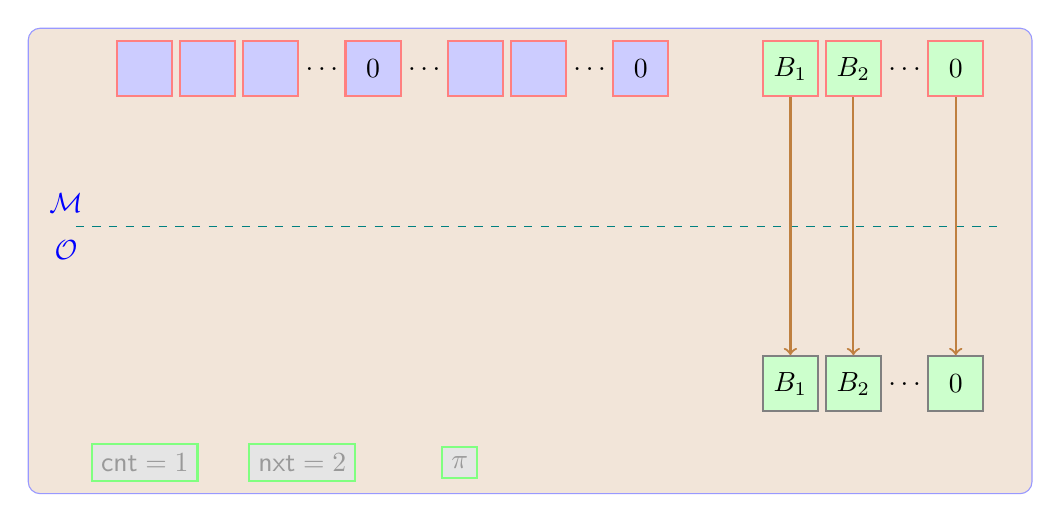
\begin{tikzpicture}
[background rectangle/.style={draw=blue!40,fill=brown!20,rounded corners=1ex},
show background rectangle,
local/.style={rectangle,draw=green!50,fill=black!10,thick},
real/.style={rectangle,draw=black!50,fill=black!20,thick},
dumm/.style={rectangle,draw=black!50,fill=magenta!20,thick},
encr/.style={rectangle,draw=red!50,fill=blue!20,thick,minimum size=7mm},
stas/.style={rectangle,draw=black!50,fill=green!20,thick,minimum size=7mm},
esta/.style={rectangle,draw=red!50,fill=green!20,thick,minimum size=7mm}]

\node at (-6,-4) (leftend) {};
\node at ( 6,-4) (rightend) {};
\node at (-6,-3.7) {{\color{blue} $\manager$}};
\node at (-6,-4.3) {\color{blue} {$\owner$}};
\draw [-,draw=teal,dashed] (leftend) to (rightend);
\node at (-5,-2)    [encr] (unoe)   {};
\node at (-4.2,-2)  [encr] (duee)   {};
\node at (-3.4,-2)  [encr] (tree)   {};
\node at (-2.75,-2)                 {$\ldots$};
\node at (-2.1,-2)  [encr] (ennee) {$0$};
\node at (-1.45,-2)                 {$\ldots$};
\node at (-0.8,-2)  [encr] (d1e)   {};
\node at ( 0.0,-2)  [encr] (d2e)   {};
\node at ( 0.65,-2)                 {$\ldots$};
\node at (1.3,-2)   [encr] (dme)   {$0$};
\node at (3.2,-2)   [esta] (se1)   {$B_1$};
\node at (4.0,-2)   [esta] (se2)   {$B_2$};
\node at (4.65,-2)                 {$\ldots$};
\node at (5.3,-2)   [esta] (sem)   {$0$};

\only<3->{
\node at (3.2,-6)   [stas] (se1d)   {$B_1$};
\node at (4.0,-6)   [stas] (se2d)   {$B_2$};
\node at (4.65,-6)                 {$\ldots$};
\node at (5.3,-6)   [stas] (semd)   {$0$};
\draw [->,draw=brown,thick] (se1.south) to (se1d.north);
\draw [->,draw=brown,thick] (se2.south) to (se2d.north);
\draw [->,draw=brown,thick] (sem.south) to (semd.north);
}

\node at (-5,-7) [local] (cnt) {\textcolor{black!40}{${\mathsf{cnt}}=1$}};
\node at (-3,-7) [local] (nxt) {\textcolor{black!40}{${\mathsf{nxt}}=2$}};
\node at (-1,-7) [local] (pi)  {\textcolor{black!40}{${\mathsf{\pi}}$}};
\end{tikzpicture}
\end{center}
\only<1-3>{{\color{white} $B_1$ is found in the Stash}}
\only<4>{\color{blue} $B_1$ is found in the Stash}
\end{frame}

\begin{frame}
\frametitle{Reading Block $B_1$ (again)}
{\color{brown} Download block in position $\pi(N+\cnt)$}
\begin{center}
\begin{tikzpicture}
[background rectangle/.style={draw=blue!40,fill=brown!20,rounded corners=1ex},
show background rectangle,
local/.style={rectangle,draw=green!50,fill=black!10,thick},
real/.style={rectangle,draw=black!50,fill=black!20,thick},
dumm/.style={rectangle,draw=black!50,fill=magenta!20,thick},
encr/.style={rectangle,draw=red!50,fill=blue!20,thick,minimum size=7mm},
stas/.style={rectangle,draw=black!50,fill=green!20,thick,minimum size=7mm},
esta/.style={rectangle,draw=red!50,fill=green!20,thick,minimum size=7mm}]

\node at (-6,-4) (leftend) {};
\node at ( 6,-4) (rightend) {};
\node at (-6,-3.7) {{\color{blue} $\manager$}};
\node at (-6,-4.3) {\color{blue} {$\owner$}};
\draw [-,draw=teal,dashed] (leftend) to (rightend);
\node at (-5,-2)    [encr] (unoe)   {};
\node at (-4.2,-2)  [encr] (duee)   {};
\node at (-3.4,-2)  [encr] (tree)   {};
\node at (-2.75,-2)                 {$\ldots$};
\node at (-2.1,-2)  [encr] (ennee) {$0$};
\node at (-1.45,-2)                 {$\ldots$};
\node at (-0.8,-2)  [encr] (d1e)   {};
\node at ( 0.0,-2)  [encr] (d2e)   {};
\node at ( 0.65,-2)                 {$\ldots$};
\node at (1.3,-2)   [encr] (dme)   {$0$};
\node at (3.2,-2)   [esta] (se1)   {$B_1$};
\node at (4.0,-2)   [esta] (se2)   {$B_2$};
\node at (4.65,-2)                 {$\ldots$};
\node at (5.3,-2)   [esta] (sem)   {$0$};

\node at (3.2,-6)   [stas] (se1d)   {$B_1$};
\node at (4.0,-6)   [stas] (se2d)   {$B_2$};
\node at (4.65,-6)                 {$\ldots$};
\node at (5.3,-6)   [stas] (semd)   {$0$};
\node at (-5,-7) [local] (cnt) {\textcolor{black!40}{${\mathsf{cnt}}=\only<1-2>{1}\only<3>{2}$}};
\node at (-3,-7) [local] (nxt) {\textcolor{black!40}{${\mathsf{nxt}}=2$}};
\node at (-1,-7) [local] (pi)  {\textcolor{black!40}{${\mathsf{\pi}}$}};
\only<-2>{\node at (-3,-3)           (ennep)   {\textcolor{magenta}{\small$\pi(N+1)$}};
\draw [->,dotted,draw=red,thick] (ennep.east) to [out=0,in=225] (d1e.west);}
\only<2>{\node at (-0.8,-6)  [encr] (d1ed)   {};
\draw [->,draw=brown,thick] (d1e.south) to (d1ed.north);}
\only<3>{
\draw [<-,draw=brown,thick] (se1.south) to (se1d.north);
\draw [<-,draw=brown,thick] (se2.south) to (se2d.north);
\draw [<-,draw=brown,thick] (sem.south) to (semd.north);
}

%%\node at (-2.1,-6)   [real] (dmed)   {$B_2$};
\end{tikzpicture}
\end{center}
\only<2>{\color{blue} No need to decrypt}
\only<3>{\color{blue} Encrypt and Upload Stash}
\end{frame}

\begin{frame}
\frametitle{Insert slide in which we argue obliviousness}
\end{frame}

\begin{frame}
\frametitle{Two issues to be dealt with}

\begin{exampleblock}{}
\begin{itemize}
\item What happens when the {\color{teal} Stash} is full?

\pause

\vskip 1cm
\item How much memory does $\owner$ need?
\begin{itemize}
\item needs to store $\color{teal}\cnt$ and $\color{teal}\nxt$: $\color{teal}\Theta(1)$ memory;
\item $\color{red} \pi$ needs $\color{red} O(N)$ memory.
\end{itemize}
\vskip .5cm
\phantom{AAA}
\end{itemize}
\end{exampleblock}
\end{frame}

\begin{frame}
\frametitle{Overflowing the Stash}
\begin{tikzpicture}
[background rectangle/.style={draw=blue!40,fill=brown!20,rounded corners=1ex},
show background rectangle,
local/.style={rectangle,draw=green!50,fill=black!10,thick},
real/.style={rectangle,draw=black!50,fill=black!20,thick,minimum size=7mm},
dumm/.style={rectangle,draw=black!50,fill=magenta!20,thick},
encr/.style={rectangle,draw=red!50,fill=blue!20,thick,minimum size=7mm},
stas/.style={rectangle,draw=black!50,fill=green!20,thick,minimum size=7mm},
esta/.style={rectangle,draw=red!50,fill=green!20,thick,minimum size=7mm}]


\node at (-6,-4) (leftend) {};
\node at ( 6,-4) (rightend) {};
\node at (-6,-3.7) {{\color{blue} $\manager$}};
\node at (-6,-4.3) {\color{blue} {$\owner$}};
\draw [-,draw=teal,dashed] (leftend) to (rightend);
\only<1-8>{
\node at (-5,-2)    [encr] (unoe)   {$B_{_{17}}$};
\node at (-4.2,-2)  [encr] (duee)   {$0$};
\node at (-3.4,-2)  [encr] (tree)   {$B_9$};
\node at (-2.75,-2)                 {$\ldots$};
\node at (-2.1,-2)  [encr] (ennee) {$0$};
\node at (-1.45,-2)                 {$\ldots$};
\node at (-0.8,-2)  [encr] (d1e)   {$B_4$};
\node at ( 0.0,-2)  [encr] (d2e)   {$B_5$};
\node at ( 0.65,-2)                 {$\ldots$};
\node at (1.3,-2)   [encr] (dme)   {$0$};
\node at (3.2,-2)   [esta] (se1)   {$B_1$};
\node at (4.0,-2)   [esta] (se2)   {$B_2$};
\node at (4.65,-2)                 {$\ldots$};
\node at (5.3,-2)   [esta] (sem)   {$0$};

\node at (-5,-7) [local] (cnt) {\textcolor{black!40}{${\mathsf{cnt}}$}};
\node at (-3,-7) [local] (nxt) {\textcolor{black!40}{${\mathsf{nxt}}$}};
}
\only<1-2>{\node at (-1,-7) [local] (pi)  {\textcolor{black!40}{${\mathsf{\pi}}$}};}
\only<2>{\node at (-1,-6) [anchor=west]{\textcolor{purple}{Randomly select a new permutation $\sigma$}};}
\only<3->{\node at (-1,-7) [local] (pi)  {\textcolor{black}{${\mathsf{\sigma}}$}};}
\only<4>{\node at (-1,-6) [anchor=west]{\textcolor{purple}{Download and decrypt first block}};
         \node at (-5,-6)  [real] (unor)   {$B_{17}$};
         \draw [->,draw=brown,thick] (unoe.south) to (unor.north);
}
\only<5>{\node at (-1,-6) [anchor=west]{\textcolor{purple}{Tag it with $\sigma(17)$ encrypt and upload}};}
\only<5-8>{\node [encr,below] at (unoe.south) {$14$};}
\only<6>{\node at (-1,-6) [anchor=west]{\textcolor{purple}{Download and decrypt first block}};
         \node at (-4.2,-6)  [real] (duer)   {$0$};
         \draw [->,draw=brown,thick] (duee.south) to (duer.north);
}
\only<7>{\node at (-1,-6) [anchor=west]{\textcolor{purple}{Tag it with $\infty$ encrypt and upload}};}
\only<7-8>{\node [encr,below] at (duee.south) {$\infty$};}
\only<8>{
    \node [encr,below] at (tree.south) {$11$};
    \node [encr,below] at (ennee.south) {$\infty$};
    \node [encr,below] at (d1e.south) {$2$};
    \node [encr,below] at (d2e.south) {$1$};
    \node [encr,below] at (dme.south) {$\infty$};
    \node [encr,below] at (se1.south) {$8$};
    \node [encr,below] at (se2.south) {$3$};
    \node [encr,below] at (sem.south) {$\infty$};
    \node at (-1,-6) [anchor=west]{\textcolor{purple}{Obliviously sort according to tags}};
}
\only<9>{
\node at (-5,-2)    [encr] (unoe)   {$B_5$};
\node at (-4.2,-2)  [encr] (duee)   {$B_4$};
\node at (-3.4,-2)  [encr] (tree)   {$B_2$};
\node at (-2.75,-2)                 {$\ldots$};
\node at (-2.1,-2)  [encr] (ennee) {};
\node at (-1.45,-2)                 {$\ldots$};
\node at (-0.8,-2)  [encr] (d1e)   {};
\node at ( 0.0,-2)  [encr] (d2e)   {$B_9$};
\node at ( 0.65,-2)                 {$\ldots$};
\node at (1.3,-2)   [encr] (dme)   {};
\node at (3.2,-2)   [esta] (se1)   {$0$};
\node at (4.0,-2)   [esta] (se2)   {$0$};
\node at (4.65,-2)                 {$\ldots$};
\node at (5.3,-2)   [esta] (sem)   {$0$};

\node at (-5,-7) [local] (cnt) {\textcolor{black!40}{$\cnt=1$}};
\node at (-3,-7) [local] (nxt) {\textcolor{black!40}{$\nxt=1$}};
}

\end{tikzpicture}

\end{frame}
\begin{frame}
\frametitle{Amortized cost per read operation}
Let us count:
\pause
\begin{itemize}[<+->]
\item each read costs
    \begin{itemize}
        \item $\color{blue} \Theta(M)$ blocks of bandwidth for the stash;
        \item $\color{blue} \Theta(1)$ blocks of bandwidth for real/dummy blocks;
    \end{itemize}
\item after $M$ reads, we shuffle
    \begin{itemize}
        \item $\color{blue} \Theta(M+N)=\Theta(N)$ blocks of bandwidth for tagging;
        \item $\color{blue} \Theta((M+N)\log (M+N))=\Theta(N\log N)$ blocks of bandwidth for sorting;
    \end{itemize}
\end{itemize}
\pause
for an amortized cost of 
$$\color{teal} \Theta\left(M+\frac{N\log N}{M}\right)$$ 
\pause
for $\color{blue} M=\sqrt{N}$ we have 
$$\color{teal} \sqrt{N}\cdot\log N.$$
\pause
Using AKS to sort. 
\pause
\hfill
{\color{brown} Huge constant}
\pause

In practice 
$\color{teal} \sqrt{N}\cdot\log^2 N.$
\end{frame}
\begin{frame}[label=firstConst]
\frametitle{In practice...\hfill
\hyperlink{recap}{\beamergotobutton{Jump ahead}}}

{\color{brown} One possible setting: }
\begin{itemize}
\item $\color{blue} N=10^6$ blocks of $4$K each for a total of $4$ Gigabytes

\item $\color{blue} M=10^3$ blocks of stash
\end{itemize}
\pause

\vskip .3cm
Resources needed:
\pause
\begin{itemize}[<+->]
\item $\manager$'s storage: $\color{teal} N+M=10^6+10^3$ blocks.

\item Cost of shuffling amortized per read operation:
        $$\color{teal} 1/2\cdot 6^2\cdot 10^3\approx 18000$$
using Batcher's sort

\item Online cost $$\color{teal}2\cdot 10^3\approx 2000$$
    
\item $\owner$'s storage
    \begin{itemize}
        \item $\cnt$ and $\nxt$ use constant storage
        \item $\pi$ requires storing $10^6$ $4$ bytes integers=4 Megabytes
    \end{itemize}
\end{itemize}
\end{frame}

\begin{frame}[label=secondConst]
\frametitle{Keep the stash in $\owner$'s memory\hfill
\hyperlink{recap}{\beamergotobutton{Jump ahead}}}

{\color{brown} Same setting: }
\begin{itemize}
\item $\color{blue} N=10^6$ blocks of $4$K each for a total of $4$ Gigabytes

\item $\color{blue} M=10^3$ blocks of stash
\end{itemize}
\pause


\vskip .3cm
Resources needed:
\pause
\begin{itemize}[<+->]
\item $\manager$'s storage: $\color{teal} N+M=10^6+10^3$ blocks

\item Cost of shuffling amortized per read operation:
        $$\color{teal} 1/2\cdot 6^2\cdot 10^3\approx 18000$$

\item Online cost: $\color{teal}2$ blocks per read
    

\item $\owner$'s storage
    \begin{itemize}
        \item $\color{teal}\cnt$ and $\color{teal}\nxt$ use constant storage
        \item $\color{teal}\pi$ requires storing $10^6$ $4$-byte integers=4 Megabytes
        \item $1000$ blocks of stash for a total of $4$ Megabytes
    \end{itemize}
\end{itemize}
\end{frame}

\section{Shuffling without Sorting}
\begin{frame}
\frametitle{Shuffling without Sorting}

\begin{itemize}[<+->]
\item {\color{blue} Input:} $\color{brown} N$ blocks stored in $\color{brown} S[1,\ldots,N]$ according to $\pi$
    \begin{itemize}
        \item Block $\color{olive} B_l$ is found in $\color{olive} [\pi(l)]$
    \end{itemize}
\item {\color{blue} Output:} $\color{brown} N$ blocks stored in $\color{brown} D[1,\ldots,N]$ according to $\sigma$
    \begin{itemize}
        \item Block $\color{olive}B_l$ will be in $\color{olive} [\sigma(l)]$
    \end{itemize}
\end{itemize}

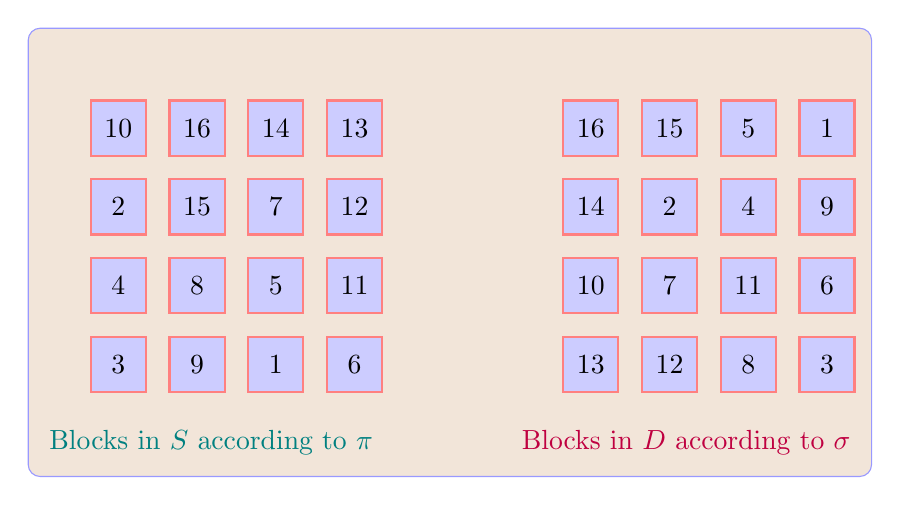
\begin{tikzpicture}
[background rectangle/.style={draw=blue!40,fill=brown!20,rounded corners=1ex},
show background rectangle,
local/.style={rectangle,draw=green!50,fill=black!10,thick},
real/.style={rectangle,draw=black!50,fill=black!20,thick,minimum size=7mm},
dumm/.style={rectangle,draw=black!50,fill=magenta!20,thick},
encr/.style={rectangle,draw=red!50,fill=blue!20,thick,minimum size=7mm},
stas/.style={rectangle,draw=black!50,fill=green!20,thick,minimum size=7mm},
esta/.style={rectangle,draw=red!50,fill=green!20,thick,minimum size=7mm}]

\def\pimatrix{{{3,4,2,10},{9,8,15,16},{1,5,7,14},{6,11,12,13}}}
\def\sigmatrix{{{13,10,14,16},{12,7,2,15},{8,11,4,5},{3,6,9,1}}}
\foreach \x in{0,1,2,3}{
    \foreach \y in{0,1,2,3}{
        %\node at (\x,\y) [encr] {\textcolor{black!40}{A}};
        %\node at (\x,\y) [encr] {\pgfmathparse{add(\x,\y)}\pgfmathresult};
        \node at (\x,\y) [encr] {\pgfmathparse{\pimatrix[\x][\y]}\pgfmathresult};
    }
}
\node at (-1,-1) [anchor=west] {\textcolor{teal}{Blocks in $S$ according to $\pi$}};
\node at (9,4){};
\only<4>{
\node at (5,-1) [anchor=west] {\textcolor{purple}{Blocks in $D$ according to $\sigma$}};
\foreach \x in{0,1,2,3}{
    \foreach \y in{0,1,2,3}{
        %\node at (\x,\y) [encr] {\textcolor{black!40}{A}};
        %\node at (\x,\y) [encr] {\pgfmathparse{add(\x,\y)}\pgfmathresult};
        \node at (\x+6,\y) [encr] {\pgfmathparse{\sigmatrix[\x][\y]}\pgfmathresult};
    }
}
}
\end{tikzpicture}
\end{frame}

\begin{frame}
\frametitle{Shuffling $N=16$}
An easy case:

\begin{tikzpicture}
[background rectangle/.style={draw=blue!40,fill=brown!20,rounded corners=1ex},
show background rectangle,
local/.style={rectangle,draw=green!50,fill=black!10,thick},
real/.style={rectangle,draw=black!50,fill=black!20,thick,minimum size=7mm},
dumm/.style={rectangle,draw=black!50,fill=magenta!20,thick},
encr/.style={rectangle,draw=red!50,fill=blue!20,thick,minimum size=7mm},
stas/.style={rectangle,draw=black!50,fill=green!20,thick,minimum size=7mm},
esta/.style={rectangle,draw=red!50,fill=green!20,thick,minimum size=7mm}] 


\def\pimatrix{{{3,4,2,10},{9,8,15,16},{1,5,7,14},{6,11,12,13}}}
\def\sigmatrix{{{13,10,14,16},{12,7,2,15},{8,11,4,5},{3,6,9,1}}}
\foreach \x in{0,1,2,3}{
    \foreach \y in{0,1,2,3}{
        %\node at (\x,\y) [encr] {\textcolor{black!40}{A}};
        %\node at (\x,\y) [encr] {\pgfmathparse{add(\x,\y)}\pgfmathresult};
        \node at (\x,\y) [encr] {\pgfmathparse{\pimatrix[\x][\y]}\pgfmathresult};
    }
}

\node at (-2,-.7) (leftend) {};
\node at (10,-.7) (rightend) {};
\node at (-2,.5)  [anchor=west] {\color{blue} $\manager$};
\node at (-2,-1.9) [anchor=west] {\color{blue} {$\owner$}};
\draw [-,draw=teal,dashed] (leftend) to (rightend);

{\node at (-1,4) [anchor=west] {\textcolor{teal}{Blocks in $S$ according to $\pi$}};}
\node at (-1,-4) [anchor=west] {};
\node at (9,4){};

\only<1>{\node at (0,5)[anchor=west]{\textcolor{purple}{Partition the $N$ blocks in $\sqrt{N}$ groups of $\sqrt{N}$}};}
\only<2>{\node at (0,5)[anchor=west]{\textcolor{purple}{Partition the $N$ destinations in $\sqrt{N}$ groups of $\sqrt{N}$}};}
\only<2->{
\foreach \x in{0,1,2,3}{
    \foreach \y in{0,1,2,3}{
        \node at (\x+6,\y) [encr] {$0$};
    }
}
}
\def\tmpmatrix{{{10,2,4,3},{16,15,8,9},{14,7,5,1},{13,12,11,6}}}

\only<3-4>{\node at (0,5)[anchor=west]{\textcolor{purple}{Download first source group}};}
\only<4>{
\foreach \y in{0,1,2,3}{
        \node at (\y,-1.5) [encr] {\pgfmathparse{\pimatrix[0][\y]}\pgfmathresult};
}
}
\only<5>{\node at (0,5)[anchor=west]{\textcolor{purple}{One block to each destination group}};}
\only<5->{\foreach \x in{0,1,2,3}{
        \node at (\x+6,0) [encr] {\pgfmathparse{\tmpmatrix[0][\x]}\pgfmathresult};
}}


\only<6-7>{\node at (0,5)[anchor=west]{\textcolor{purple}{Download second source group}};}
\only<7>{
\foreach \y in{0,1,2,3}{
        \node at (\y,-1.5) [encr] {\pgfmathparse{\pimatrix[1][\y]}\pgfmathresult};
}
}
\only<8>{\node at (0,5)[anchor=west]{\textcolor{purple}{One block to each destination group}};}
\only<8->{
\foreach \x in{0,1,2,3}{
        \node at (\x+6,1) [encr] {\pgfmathparse{\tmpmatrix[1][\x]}\pgfmathresult};
}}

\only<9-10>{\node at (0,5)[anchor=west]{\textcolor{purple}{Download second source group}};}
\only<10>{
\foreach \y in{0,1,2,3}{
        \node at (\y,-1.5) [encr] {\pgfmathparse{\pimatrix[2][\y]}\pgfmathresult};
}
}
\only<11>{\node at (0,5)[anchor=west]{\textcolor{purple}{One block to each destination group}};}
\only<11->{
\foreach \x in{0,1,2,3}{
        \node at (\x+6,2) [encr] {\pgfmathparse{\tmpmatrix[2][\x]}\pgfmathresult};
}}

\only<12-13>{\node at (0,5)[anchor=west]{\textcolor{purple}{Download second source group}};}
\only<13>{
\foreach \y in{0,1,2,3}{
        \node at (\y,-1.5) [encr] {\pgfmathparse{\pimatrix[3][\y]}\pgfmathresult};
}
}
\only<14>{\node at (0,5)[anchor=west]{\textcolor{purple}{One block to each destination group}};}
\only<14->{
\foreach \x in{0,1,2,3}{
        \node at (\x+6,3) [encr] {\pgfmathparse{\tmpmatrix[3][\x]}\pgfmathresult};
}}

\only<15>{\node at (0,5)[anchor=west]{\textcolor{purple}{Each block in the right destination group}};}
\only<16->{\node at (0,5)[anchor=west]{\textcolor{purple}{Download each group and upload in correct position}};}


\only<17>{
\foreach \y in{0,1,2,3}{
        \node at (\y,-1.5) [encr] {\pgfmathparse{\tmpmatrix[\y][0]}\pgfmathresult};
}}
\only<18->{
\foreach \x in{0,1,2,3}{
        \node at (6,\x) [encr] {\pgfmathparse{\sigmatrix[0][\x]}\pgfmathresult};
}}

\only<19>{
\foreach \y in{0,1,2,3}{
        \node at (\y,-1.5) [encr] {\pgfmathparse{\tmpmatrix[\y][1]}\pgfmathresult};
}}
\only<20->{
\foreach \x in{0,1,2,3}{
        \node at (7,\x) [encr] {\pgfmathparse{\sigmatrix[1][\x]}\pgfmathresult};
}}

\only<20>{
\foreach \y in{0,1,2,3}{
        \node at (\y,-1.5) [encr] {\pgfmathparse{\tmpmatrix[\y][2]}\pgfmathresult};
}}
\only<21->{
\foreach \x in{0,1,2,3}{
        \node at (8,\x) [encr] {\pgfmathparse{\sigmatrix[2][\x]}\pgfmathresult};
}}

\only<22>{
\foreach \y in{0,1,2,3}{
        \node at (\y,-1.5) [encr] {\pgfmathparse{\tmpmatrix[\y][3]}\pgfmathresult};
}}
\only<23->{
\foreach \x in{0,1,2,3}{
        \node at (9,\x) [encr] {\pgfmathparse{\sigmatrix[3][\x]}\pgfmathresult};
}}

\only<24->{\node at (5,4) [anchor=west] {\textcolor{teal}{Blocks in $D$ according to $\sigma$}};}

\end{tikzpicture}
\end{frame}

\begin{frame}
\frametitle{Analysis of Shuffling Algorithm}

\begin{itemize}[<+->]

\item {\color{blue} Obliviousness}: access pattern independent of $\pi,\sigma$
    \begin{itemize}
        \item download each source group
        \item upload one block to each destination group in the next available empty location
        \item download each destination group
        \item upload each destination group
    \end{itemize}
\vskip 1cm
\item {\color{blue} bandwidth}: $4N$

        each block
    \begin{itemize}
        \item downloaded exactly twice
        \item uploaded exactly twice
    \end{itemize}

\vskip 1cm

\item {\color{blue} Luck}: so much!!!
    \begin{itemize}
        \item {\color{red} each source group} contains {\color{red} exactly one block} for 
              {\color{red} each destination group} under $\sigma$
    \end{itemize}
\end{itemize}
\end{frame}

\begin{frame}
\frametitle{Efficient Shuffling: CacheShuffleRoot}

{\em \color{brown} when you know you are not going to be lucky, just randomize}

\pause

\begin{itemize}[<+->]
\item {\color{purple} Randomly partition} {\color{red}destination} array in $\color{blue} (1+2\epsilon)\sqrt{N}$ groups
\begin{itemize}
\item Each group has size at most $\color{blue} (1-\epsilon)\sqrt{N}$, except with negligible probability
\end{itemize}
\vskip .2cm
\item {\color{purple} Spray phase}
\begin{itemize}
    \item Download each {\color{red}source group} and {\color{purple} spray} exactly {\color{red} one} block
            to each {\color{red} destination group}
    \item if none available, {\color{purple} spray a dummy block}
    \item if more than one available, {\color{purple} spray exactly one} and 
        {\color{purple}store} the extra blocks in {\color{purple} local cache}
\end{itemize}
\vskip .2cm
\item {\color{purple} Recalibrate phase}
    \begin{itemize}
        \item download each {\color{red} destination group}
        \item remove dummies
        \item add blocks found in local cache
        \item upload in correct order
    \end{itemize}
\end{itemize}
\end{frame}

\begin{frame}
\frametitle{Analysis of CacheShuffleRoot}

\begin{itemize}[<+->]
 \item {\color{olive} bandwidth}: $\color{blue} (4+\epsilon)N$ blocks
    \begin{itemize}
        \item each {\color{blue} real} block is downloaded exactly twice and uploaded exactly twice
        \item each {\color{teal} dummy} block is uploaded exactly once and downloaded exactly once
        \item number of {\color{teal} dummy} blocks is at most $\epsilon\cdot N$ except with negligible probability
    \end{itemize}

 \item {\color{olive} Obliviousness}: access pattern is fixed for all executions
    \begin{itemize}
        \item download each source group
        \item upload one block to each destination group
        \item when done, download and upload each destination group
    \end{itemize}

  \item {\color{olive} $\manager$'s storage}: $\color{blue}\Theta(N)$

    \item {\color{olive} $\owner$'s storage}
    \begin{itemize}
        \item next slide
    \end{itemize}
\end{itemize}
\end{frame}

\begin{frame}
\frametitle{Analysis of CacheShuffleRoot: $\owner$'s storage}

{\color{brown} Intuition}

\begin{itemize}[<+->]
\item  $\owner$'s keeps a cache for each of the $\color{blue}(1+2\epsilon)\sqrt{N}$ destination groups
\item each cache has arrival rate $\approx(1-2\epsilon)$
\item departure rate $1$
\item each cache is expected to hold a constant number of blocks
\item total $\owner$'s storage is $\Theta(\sqrt{N})$ except with negligible probability
\end{itemize}

\pause
{\color{brown} Formal argument}
\begin{itemize}[<+->]
\item cache sizes are not independent so cannot use Chernoff bound
\item prove negative association and then use Chernoff bound 
\end{itemize}
\end{frame}

\section{A second construction}
\begin{frame}
\frametitle{Keep the stash in $\owner$'s memory and use CacheShuffleRoot}

{\color{brown} Same setting: }
\begin{itemize}
\item $\color{blue} N=10^6$ blocks of $4$K each for a total of $4$ Gigabytes

\item $\color{blue} M=10^3$ blocks of stash
\end{itemize}
\pause


\vskip .3cm
Resources needed:
\pause
\begin{itemize}[<+->]
\item $\manager$'s storage: $\color{teal} N+M=10^6+10^3$ blocks

\item Cost of shuffling amortized per read operation:
        $$\color{teal} 4\cdot 10^3\approx 4000$$

\item Online cost: $\color{teal}2$ blocks per read
    

\item $\owner$'s storage
    \begin{itemize}
        \item $\color{teal}\cnt$ and $\color{teal}\nxt$ use constant storage
        \item $\color{teal}\pi$ requires storing $10^6$ $4$-byte integers=4 Megabytes
        \item $1000$ blocks of stash for a total of $4$ Megabytes
    \end{itemize}
\end{itemize}
\end{frame}

\begin{frame}[label=recap]
\frametitle{Where are we now?}

\begin{columns}[t]
\begin{column}{5cm}
\begin{block}{\hyperlink{zeroConst<10>}{\beamergotobutton{Construction -1}}\hfill Keep It}
\begin{itemize}
\item $\color{blue} \manager$'s storage: $0$
\item $\color{blue} \owner$'s storage: $\color{magenta}N$
\item {\color{blue} bandwidth} $0$
\end{itemize}
\end{block}
\end{column}
\begin{column}{5cm}
\begin{block}{\hyperlink{zeroConst<10>}{\beamergotobutton{Construction 0}}\hfill Download It}
\begin{itemize}
\item $\color{blue} \manager$'s storage: $\color{magenta}N$
\item $\color{blue} \owner$'s storage: $\color{magenta}1$
\item {\color{blue} bandwidth} $\color{magenta}N$
\end{itemize}
\end{block}
\end{column}
\end{columns}

\noindent
\begin{columns}[t]
\begin{column}{5cm}
\begin{block}{\hyperlink{firstConst<8>}{\beamergotobutton{Construction 1}}\hfill Download Stash}
\begin{itemize}
\item $\color{blue} \manager$'s storage: $\color{magenta}N+\sqrt{N}$
\item $\color{blue} \owner$'s storage: $\color{magenta}1$
\item {\color{blue} Online Comm.} $\color{magenta} O(\sqrt{N})$
\item {\color{blue} Am. Comm.} $\color{magenta} O(\sqrt{N}\cdot \log N)$
\end{itemize}
\end{block}
\end{column}
\begin{column}{5cm}

\begin{block}{\hyperlink{secondConst<9>}{\beamergotobutton{Construction 2}}\hfill Keep Stash}
\begin{itemize}
\item $\color{blue} \manager$'s storage: $\color{magenta}N+\sqrt{N}$
\item $\color{blue} \owner$'s storage: $\color{magenta}\sqrt{N}$
\item {\color{blue} Online Comm.} $\color{magenta} 1$
\item {\color{blue} Am. Comm.} $\color{magenta} O(\sqrt{N}\cdot \log N)$
\end{itemize}
\end{block}
\end{column}
\end{columns}
\end{frame}

\begin{frame}
\frametitle{Download and Keep Stash}

\begin{itemize}[<+->]
\item Use a cache (the {\color{teal} Stash}) to hide the repetition  pattern
\item How does $\color{olive}\owner$ hide access to the {\color{teal} Stash}?
    \begin{itemize}
        \item Use an ORAM!
        \item We only have two possible ORAMs:
        \item {\color{blue} Download Stash} uses the {\color{blue} Download It} ORAM
            to manage the {\color{teal} Stash}
        \item {\color{blue} Keep Stash} uses the {\color{blue} Keep It} ORAM
            to manage the {\color{teal} Stash}
    \end{itemize}
\end{itemize}

\pause
\alert{But now we have more ORAMs!!!}
\end{frame}

\section{A Recursive Construction}
\begin{frame}
\begin{center}
\begin{tikzpicture}
[background rectangle/.style={draw=blue!40,fill=brown!20,rounded corners=1ex},
show background rectangle,
local/.style={rectangle,draw=green!50,fill=black!10,thick,minimum size=7mm},
real/.style={rectangle,draw=black!50,fill=black!20,thick,minimum size=7mm},
dumm/.style={rectangle,draw=black!50,fill=magenta!20,thick,minimum size=7mm},
encr/.style={rectangle,draw=red!50,fill=blue!20,thick,minimum size=7mm},
stas/.style={rectangle,draw=black!50,fill=green!20,thick,minimum size=7mm},
esta/.style={rectangle,draw=red!50,fill=green!20,thick,minimum size=7mm}]

\node at (-6,-4) (leftend) {};
\node at ( 5,-4) (rightend) {};
\node at (-6,-3.7) {{\color{blue} $\manager$}};
\node at (-6,-4.3) {\color{blue} {$\owner$}};
\draw [-,draw=teal,dashed] (leftend) to (rightend);
\node at (-5,0) [anchor=west] {};

\only<1>{
\node at (-6,   -5) [anchor=west] {\textcolor{olive}{$N$ blocks of data}};
\node at (-6,   -6) [real] (unoe)   {$B_1$};
\node at (-5.2, -6) [real] (duee)   {$B_2$};
\node at (-4.4, -6) [real] (tree)   {$B_3$};
\node at (-3.75,-6)                 {$\ldots$};
\node at (-3.1,- 6) [real] (ennee)  {$B_N$};
}

\only<2-6>{\node at (2.6,   0) [anchor=west] {\textcolor{olive}{$N+\rho N$}};}
\only<2->{
\node at (-6,    0) [encr] (unoe) {};
\node at (-5.2,  0) [encr] (duee) {};
\node at (-4.4,  0) [encr] (tree) {};
\node at (-3.75, 0)               {$\ldots$};
\node at (-3.1,  0) [encr] (ennee){};
\node at (-2.45, 0)               {$\ldots$};
\node at (-1.8,  0) [encr] (d1e)  {};
\node at (-1.0,  0) [encr] (d2e)  {};
\node at (-0.3,  0)               {$\ldots$};
\node at ( 0.4,  0)  [encr] (dme) {};
}

\only<2>{
\node at (-6,   -5) [anchor=west] {\textcolor{olive}{$\rho N$ blocks of stash}};
\node at (-6,   -6) [real] (unoe) {$0$};
\node at (-5.2, -6) [real] (duee) {$0$};
\node at (-4.4, -6) [real] (tree) {$0$};
\node at (-3.75,-6)               {$\ldots$};
\node at (-3.1, -6) [real] (ennee){$0$};
}


\only<3-6>{\node at (2.6,  -1) [anchor=west] {\textcolor{olive}{$\rho N+\rho^2 N$}};}
\only<3->{
\node at (-6,   -1) [encr] (unoe) {};
\node at (-5.2, -1) [encr] (duee) {};
\node at (-4.4, -1) [encr] (tree) {};
\node at (-3.75,-1)               {$\ldots$};
\node at (-3.1, -1) [encr] (ennee){};
}

\only<3>{
\node at (-6,   -5) [anchor=west] {\textcolor{olive}{$\rho^2 N$ blocks of stash}};
\node at (-6,   -6) [real] (unoe)   {$0$};
\node at (-5.2, -6) [real] (duee)   {$0$};
\node at (-4.4, -6)                  {$\ldots$};
\node at (-3.75,-6) [real] (tree)   {$0$};
}

\only<4-6>{\node at (2.6,  -2) [anchor=west] {\textcolor{olive}{$\rho^2 N+\rho^3 N$}};}
\only<4->{
\node at (-6,   -2) [encr] (unoe) {};
\node at (-5.2, -2)               {$\ldots$};
\node at (-4.4, -2) [encr] (tree) {};
}

\only<4-5>{\node at (-6,   -5) [anchor=west] {\textcolor{olive}{$\rho^3 N$ blocks of stash}};}
\only<4->{
\node at (-6,   -6) [real] (unoe) {$0$};
\node at (-5.3, -6)               {$\ldots$};
\node at (-4.6, -6) [real] (tree) {$0$};
}
\only<6>{\node  at (-2,   -5) [anchor=west] {\textcolor{purple}{$\rho=N^{-1/6}$}};}
\only<6->{\node at (-6,   -5) [anchor=west] {\textcolor{olive}{$\sqrt{N}$ blocks of stash}};}
\only<7->{\node at (2.6,  -2) [anchor=west] {\textcolor{olive}{$N^{2/3}+N^{1/2}$}};}
\only<7->{\node at (2.6,  -1) [anchor=west] {\textcolor{olive}{$N^{5/6}+N^{2/3}$}};}
\only<7->{\node at (2.6,   0) [anchor=west] {\textcolor{olive}{$N+N^{5/6}$}};}
\only<8->{
\node at (-0.5, -5.4) [anchor=west] {\textcolor{blue}{Position Map}};
\node at (1.5,  -6) [local] (cnt) {\textcolor{black!40}{$({\mathsf{lev_i,pos_i}})\ i=1,\ldots,N$}};
\node at (-3.8,  -6) [anchor=west] {\textcolor{blue}{Level 0}};
\node at ( 1.0,  -2) [anchor=west] {\textcolor{blue}{Level 1}};
\node at ( 1.0,  -1) [anchor=west] {\textcolor{blue}{Level 2}};
\node at ( 1.0,   0) [anchor=west] {\textcolor{blue}{Level 3}};
}
\end{tikzpicture}
\end{center}
\end{frame}

\begin{frame}
\frametitle{$3$-level ORAM: Querying}
{\color{purple}Querying $ B_q$}
\begin{itemize}[<+->]
\item retrieve $\color{olive}({\mathsf{lev_q,pos_q}})$ from local memory;
\item if $\color{olive}{\mathsf{lev_q}}\ne 0$ 
    \begin{itemize}
        \item for all $\color{olive} l\ne{\mathsf{lev_q}}$, $\color{purple}\owner$ asks 
            for the next {\color{teal} dummy} in level $l$;
        \item asks for block in ${\color{olive} \mathsf{pos_q}}$ from level ${\color{olive} \mathsf{lev_q}}$;
        \item $B_q$ is then stored in level $0$ and ${\color{olive}(\mathsf{lev_q,pos_q}})$ is updated;
    \end{itemize}
    \item else
    \begin{itemize}
        \item for $l=1,2,3$, $\color{purple}\owner$ asks for the next {\color{teal} dummy} in level $l$;
        \item block $B_q$ is retrieved from local stash (level 0);
    \end{itemize}
\end{itemize}
\end{frame}

\begin{frame}
\frametitle{3-level ORAM: Analysis}
\begin{itemize}[<+->]
\item at the start only level $3$ contains {\color{teal} real blocks};
\item {\color{blue} the local stash is full after $N^{1/2}$ queries}
\begin{itemize}
\item it is shuffled with the level $1$ of size $N^{2/3}$;
\item each shuffle costs $4 N^{2/3}$
\item over $N$ queries, it happens $N^{1/2}$ times
\item total cost: $4\cdot N^{7/6}$
\end{itemize}
\item {\color{blue} level $1$ is full after $N^{2/3}$ queries}
\begin{itemize}
\item it is shuffled with the level $2$ of size $N^{5/6}$;
\item each shuffle costs $4 N^{5/6}$
\item over $N$ queries, it happens $N^{1/3}$ times
\item total cost: $4\cdot N^{7/6}$
\end{itemize}
\item {\color{blue} level $2$ is full after $N^{5/6}$ queries}
\begin{itemize}
\item it is shuffled with the level $3$ of size $N$;
\item each shuffle costs $4 N$
\item over $N$ queries, it happens $N^{1/6}$ times
\item total cost: $4\cdot N^{7/6}$
\end{itemize}
\item {\color{blue} Over $N$ queries, the cost is $12\cdot N^{7/6}$}
\begin{itemize}
\item {\color{magenta} each query has an amortized cost of $12N^{1/6}$ blocks;}
\end{itemize}
\end{itemize}
\end{frame}

\begin{frame}
\frametitle{3-level ORAM: in practice}

{\color{brown} Same setting: }
\begin{itemize}
\item $\color{blue} N=10^6$ blocks of $4$K each for a total of $4$ Gigabytes

\item $\color{blue} M=10^3$ blocks of stash for a total of $4$ Megabytes
\end{itemize}
\pause


\vskip .3cm
Resources needed:
\pause
\begin{itemize}[<+->]
\item $\manager$'s storage: $\color{teal} 10^6+2\cdot 10^5+2\cdot 10^4+10^3=
1,221,000$ blocks

\item Cost of shuffling amortized per read operation:
        $$\color{teal} 4\cdot 10^3\approx 120$$

\item Online cost: $\color{teal}3$ blocks downloaded
    

\item $\owner$'s storage
    \begin{itemize}
        \item $\color{teal}\cnt$ and $\color{teal}\nxt$ use constant storage
        \item {\color{teal}position map} requires storing $10^6$
            $6$-byte integers $\approx 4$ Megabytes
        \item $1000$ blocks of stash for a total of $4$ Megabytes
    \end{itemize}
\end{itemize}
\end{frame}

\begin{frame}
\frametitle{Why stop at 3 levels?}

$\owner$'s memory $\approx\sqrt{N}$ 
\begin{itemize}[<+->]
\item set $\color{teal}\rho=1/2$
\item $\color{teal}1/2\log_2 N$ levels with 
    \begin{itemize}
    \item $\color{teal}N+N/2$ blocks
    \item $\color{teal}N/2+N/4$ blocks
    \item $\color{teal}\ldots$
    \item $\color{teal}3\sqrt{N}$ blocks
    \end{itemize}
\item Amortized bandwidth $\color{red} 0.55\cdot\log_2 N$ 
    \begin{itemize}
        \item For $\color{teal}N=10^6$, {\color{red} 21 Blocks}
    \end{itemize}
\item OnLine bandwidth: {\color{red} $1$ Block}
\end{itemize}

\pause

\begin{block}{Techniques to reduce bandwidth}
\begin{itemize}
{\color{brown}
\item XOR Technique
\item Homomorphic Selection
\item Compression via Polynomial Interpolation
}
\end{itemize}
\end{block}
\end{frame}

\begin{frame}
\frametitle{The XOR technique to reduce bandwidth}

{\color{purple} $l$-level ORAM}
\vskip 1cm
\begin{itemize}[<+->]
\item when asking for $\color{brown}B_q$,
    $\color{purple}\owner$ asks one block {\color{blue} for each level}
\item at most one block is {\color{blue}real}
\item suppose $\color{purple}\owner$ can compute locally the $\color{blue} l-1$ dummy blocks requested
    \begin{itemize}
        \item $\color{purple}\manager$ instead of sending all $\color{blue} l$ blocks individually,
{\color{red} xors} them together and sends the result to $\color{purple}\owner$
        \item $\color{purple}\owner$ computes the $\color{blue} l-1$ dummy blocks and 
{\color{red} xors} them with
        the block received from $\color{purple}\manager$
    \end{itemize}
\end{itemize}
\end{frame}

\begin{frame}
{\color{brown}\bf Assumption:} {\em suppose $\color{purple}\owner$ can compute any {\color{teal} dummy} block without interacting with  $\color{purple}\manager$}

\begin{itemize}
\item each block uniquely identified by $\color{teal} (\mathsf{l,pos})$
\item a {\color{teal}dummy} block is an AES-ECB encryption of $0^{\mathsf{len}}$  
\item using key ${\color{brown}\cal F}({\color{olive} K},\color{teal}(\mathsf{l,pos})$
    \begin{itemize}
        \item ${\color{brown}\cal F}$ is a pseudorandom function
        \item ${\color{olive} K}$ is a randomly chosen seed private to $\owner$
    \end{itemize}
\end{itemize}
\end{frame}

\section{Lower Bounds}
\begin{frame}
\frametitle{Some Theory}
{\color{brown}\bf A Taxonomy}

\begin{itemize}
\item {\color{brown}\bf OnLine} vs {\color{brown}\bf OffLine ORAM}
    \begin{itemize}
        \item In an {\color{brown}\bf OnLine} ORAM, all requests come one at the time and must be satisfied before the next one
        \item in an {\color{brown}\bf OffLine} ORAM, all requests come together 
    \end{itemize}
\item {\color{brown}\bf BallsAndBins}
    \begin{itemize}
        \item Blocks are atomic and opaque blobs of data
    \end{itemize}
\item {\color{brown}\bf Passive} vs {\color{brown} \bf Active} $\color{purple}\manager$
    \begin{itemize}
        \item A {\color{brown}\bf Passive} $\color{purple}\manager$ only moves data 
        \item An {\color{brown}\bf Active} $\color{purple}\manager$ can perform computation on data 
    \begin{itemize}
        \item  The {\color{blue}\bf XOR technique} requires an {\color{brown}\bf Active} $\color{purple}\manager$
    \end{itemize}
    \end{itemize}
\end{itemize}
\end{frame}

\begin{frame}

\frametitle{What we know in the asymptotic world}

\begin{itemize}[<+->]
\item All the following require $\color{blue}\bf\Omega(\log N)$
\begin{itemize}
\item {\color{brown}\bf BallsAndBins} and {\color{brown}\bf OffLine} with {\color{brown}\bf Passive } $\color{purple}\manager$
\item {\color{brown}\bf NonBallsAndBins} and {\color{brown}\bf OnLine} with {\color{brown}\bf Passive } $\color{purple}\manager$
\end{itemize}
\vskip .3cm

\item There are $\color{blue}\bf\tilde O(\log N)$ {\color{brown}\bf OnLine} ORAM in the Balls and Bins model with  {\color{brown}\bf Passive } $\color{purple}\manager$
\vskip .3cm

\item There are $\color{blue}\bf o(\log N)$ {\color{brown}\bf OnLine} ORAM with {\color{brown}\bf  Active } $\color{purple}\manager$
\vskip .3cm

\item Proving lower bound for 
{\color{brown}\bf Non-BallsAndBins} and {\color{brown}\bf OffLine} with {\color{brown} \bf Passive} $\color{purple}\manager$
would give a superlinear lower bound for sorting circuits.
\end{itemize}
\end{frame}
}

\section{Differential Privacy}
\begin{frame}[label=dp]
\frametitle{Differential Privacy \hfill \hyperlink{GO<2>}{\beamergotobutton{ORAM}}}

\begin{block}{$(\epsilon,\delta)$-Differential Privacy}
\begin{itemize}
\item {\color{blue} $\manager$ stores $n$ blocks of memory.}
\item {\color{blue} Every time $\owner$ wants a block, he asks $\manager$ one or more blocks.}

{\color{olive}
\item Security notion:
\begin{itemize}
\color{olive}
\item For any two block sequences $\color{teal} \mathbb{B}=B_1,\ldots,B_n$ and 
                                    $\color{magenta} \mathbb{C}=C_1,\ldots,C_n$
\item For any two access sequences $\color{teal}    i_1,\ldots,i_l$ and 
                                   $\color{magenta} j_1,\ldots,j_l$
{\color{blue}\bf that differ in one position}
\begin{itemize}
\color{olive}
    \item performing access $\color{teal}    i_1,\ldots,i_l$ on
                $\color{teal} \mathbb{B}=B_1,\ldots,B_n$;
    \item performing access $\color{magenta} j_1,\ldots,j_l$ on
                $\color{magenta} \mathbb{C}=C_1,\ldots,C_n$
\end{itemize}
\end{itemize}
    generate the same distribution of accesses to the data stored by $\manager$
}
\end{itemize}
\end{block}
\pause
For every predicate $A$
\begin{align*}
\text{\rm Prob}[&\mathtt{view}\leftarrow\mathtt{View}({\color{teal}I,\mathbb{B}}):
    A(\mathtt{view})=1]\\ & \leq e^{\color{blue} \epsilon}\cdot
  \text{\rm Prob}[\mathtt{view}\leftarrow\mathtt{View}({\color{magenta}J,\mathbb{C}}):
    A(\mathtt{view})=1]+{\color{blue} \delta}
\end{align*}
\end{frame}

\begin{frame}
\frametitle{Differential Privacy}

\begin{itemize}[<+->]
\item it protects only \alert{individual} accesses
\item if the probability of an access
is larger than $\color{blue}1/e^{\epsilon}$ no guarantee is given
\item it protects {\color{purple} unusual accesses}
\item how unusual?
    \begin{itemize} \item it depends on $\color{blue}\epsilon$ \end{itemize}
\item no protection is offered for {\color{brown}high-probability} accesses
    \begin{itemize}
        \item {\color{olive} nothing is lost: my daily routine is public}
    \end{itemize}
\item I really want to protect {\color{purple} unusual accesses}
    to documents that might reveal something

    \begin{itemize}
        \item I am checking my medical records from some time ago...
    \end{itemize}
\end{itemize}



\end{frame}

\begin{frame}
\begin{center}
\begin{tikzpicture}
[background rectangle/.style={draw=blue!40,fill=brown!20,rounded corners=1ex},
show background rectangle,
local/.style={rectangle,draw=green!50,fill=black!10,thick,minimum size=7mm},
real/.style={rectangle,draw=black!50,fill=black!20,thick,minimum size=7mm},
dumm/.style={rectangle,draw=black!50,fill=magenta!20,thick,minimum size=7mm},
encr/.style={rectangle,draw=red!50,fill=blue!20,thick,minimum size=7mm},
stas/.style={rectangle,draw=black!50,fill=green!20,thick,minimum size=7mm},
esta/.style={rectangle,draw=red!50,fill=green!20,thick,minimum size=7mm}]

\node at (-6,-4) (leftend) {};
\node at ( 5,-4) (rightend) {};
\node at (-6,-3.7) {{\color{blue} $\manager$}};
\node at (-6,-4.3) {\color{blue} {$\owner$}};
\draw [-,draw=teal,dashed] (leftend) to (rightend);
\node at (-5,0) [anchor=west] {};

\only<1>{
\node at (-6,   -5) [anchor=west] {\textcolor{olive}{$N$ blocks of data}};
\node at (-6,   -6) [real] (unoe)   {$B_1$};
\node at (-5.2, -6) [real] (duee)   {$B_2$};
\node at (-4.4, -6) [real] (tree)   {$B_3$};
\node at (-3.75,-6)                 {$\ldots$};
\node at (-3.1,- 6) [real] (ennee)  {$B_N$};
\node at (-6,    0) {};
}

\only<2-6>{
\node at (2.2,   0) [anchor=west] {\textcolor{olive}{$N$ encrypted blocks}};
\node at (2.2,  -1) [anchor=west] {\textcolor{olive}{probability $p$}};
}
\only<2->{
\node at (-6,    0) [encr] (unoe) {$B_1$};
\node at (-5.2,  0) [encr] (duee) {$B_2$};
\node at (-4.4,  0) [encr] (tree) {$B_3$};
\node at (-3.75, 0)               {$\ldots$};
\node at (-3.1,  0) [encr] (ennee){$B_N$};
\node at (-3.1,- 6) {};
}

\only<3->{
\node at (-6,   -5) [anchor=west] {\textcolor{olive}{Stash}};
\node at (-3.2, -5) [real] (duee) {$B_7$};
\node at (-2.4, -5) [real] (tree) {$B_{9}$};
\node at (-1.75,-5)               {$\ldots$};
\node at (-1.1, -5) [real] (ennee){$B_{N-2}$};
\node at ( 2.2, -5) [anchor=west] {\textcolor{olive}{$pN$ expected blocks}};
}
\end{tikzpicture}
\end{center}
\end{frame}

\begin{frame}
\frametitle{Querying for $B_i$}
\begin{block}{Download Phase}
\begin{itemize}[<+->]
\item {\color{blue} if $B_i$ is found in the stash:}
    \begin{itemize}
        \item return it 
        \item remove it from the stash
        \item ask $\color{purple} \manager$ for a random block and then discard it
    \end{itemize}
\item{\color{blue} if $B_i$ is not found in the stash:}
    \begin{itemize}
        \item ask $\color{purple} \manager$ for $\color{purple} B_i$
    \end{itemize}
\end{itemize}
\end{block}
\begin{block}{Overwrite Phase}
\begin{itemize}[<+->]
\item Toss a coin with probability $\color{olive} (p,1-p)$
\item if head
    \begin{itemize}
        \item add $\color{purple} B_i$ to stash
        \item ask $\color{purple} \manager$ for a randomly selected block, 
        re-encrypt it and upload to the same location
    \end{itemize}
\item if tail
    \begin{itemize}
        \item download $\color{purple} B_i$ from $\color{purple} \manager$
        \item decrypt and re-encrypt and upload it to the same location
    \end{itemize}
\end{itemize}
\end{block}
\end{frame}

\begin{frame}
\frametitle{Analysis}
\begin{itemize}[<+->]
\item Two blocks of communication
\item $p=\omega(\log n/n)$ with $\omega(\log n)$ client memory
\item $\epsilon=\Theta(\log n)$
\end{itemize}


\pause

\begin{theorem}
For any $\color{brown}\epsilon \ge 0$, any {\sf{DP-RAM}} with error probability $\color{brown}\alpha \ge 0$
in the BallsAndBins model and a client that stores at most $c$ blocks must operate on
$$\color{purple}
\Omega\left(\log_c \left(\frac{(1-\alpha) \cdot n}{e^\epsilon}\right)\right)
$$
records.

In the non-BallsAndBins the bound is 
$$\color{purple}
\Omega\left(\frac{b}{w}\log \frac{nb}{c}\right)
$$
for any constant $\epsilon$, $\delta\leq 1/3$ and error probability $1/3$.

\end{theorem}

\end{frame}

\section{Where are we?}
\begin{frame}
\frametitle{Conclusions}
\begin{itemize}[<+->]
\item{\color{blue} \bf Leaking the access pattern can be dangerous}
\item {\color{purple} Obliviousness}: a strong security notion
\begin{itemize}
    \item {\color{brown} requires $>20$x overhead for $4$ Giga of data}
\end{itemize}
\item {\color{purple} Differential Privacy}: a weaker security notion
\begin{itemize}
    \item {\color{brown} very efficient }
    \item {\color{brown} suitable only for specific applications}
\end{itemize}
\item Other security notions?
\item Better analysis under reasonable assumptions for access distributions?
Zipf?

\end{itemize}
\pause

\pause
{\small 
{\tt{https://github.com/giuper/talks/nonTechnical/oramTutorial.pdf}}
}
\end{frame}



%%\nocite{*}
%%\bibliographystyle{abbrv}
%%\bibliography{biblio}

\begin{frame}
\frametitle{The original papers}

\begin{thebibliography}{10}
\bibitem{G:87}
O.~Goldreich.
\newblock {Towards a Theory of Software Protection and Simulation by Oblivious RAMs}.
\newblock In {\em STOC}, 1987.

\bibitem{O:90}
R.~Ostrovsky.
\newblock Efficient computation on oblivious {RAM}s.
\newblock In {\em STOC}, pages 514--523, 1990.

\bibitem{GO:96}
O.~Goldreich and R.~Ostrovsky.
\newblock {Software Protection and Simulation on Oblivious RAMs}.
\newblock {\em J. ACM}, 43(3), 1996.
\end{thebibliography}
\end{frame}

\begin{frame}
\frametitle{Asymptotics}

\begin{thebibliography}{10}
\bibitem{AKL18}
G.~Asharov, I.~Komargodski, W.-K. Lin, K.~Nayak, E.~Peserico, and E.~Shi.
\newblock Opt{ORAM}a: Optimal oblivious {RAM}.
\newblock Cryptology ePrint Archive, Report 2018/892.

\bibitem{full-version}
S.~Patel, G.~Persiano, M.~Raykova, and K.~Yeo.
\newblock Pan{ORAM}a: Oblivious {RAM} with logarithmic overhead.
\newblock Cryptology ePrint Archive, Report 2018/373, 2018.
\newblock https://eprint.iacr.org/2018/373.
\newblock FOCS '18.
\end{thebibliography}

\vfill
{\color{brown} \bf Constant client memory}
\end{frame}

\begin{frame}
\frametitle{Efficient constructions for large blocks}
\begin{thebibliography}{10}
\bibitem{pathORAM}
E.~Stefanov, M.~van Dijk, E.~Shi, C.~Fletcher, L.~Ren, X.~Yu, and S.~Devadas.
\newblock {Path ORAM: An Extremely Simple Oblivious RAM Protocol}.
\newblock In {\em CCS '13}, pages 299--310, 2013.
\bibitem{DDF16}
S.~Devadas, M.~van Dijk, C.~W. Fletcher, L.~Ren, E.~Shi, and D.~Wichs.
\newblock {Onion ORAM: A constant bandwidth blowup oblivious RAM}.
\newblock In {\em TCC}, pages 145--174, 2015.
\bibitem{MMB15}
T.~Moataz, T.~Mayberry, and E.-O. Blass.
\newblock {Constant communication ORAM with small blocksize}.
\newblock In {\em CCS}, pages 862--873, 2015.
\end{thebibliography}

\vfill
{\color{brown} \bf polylog(n)-bit blocks}

\end{frame}

\begin{frame}
\frametitle{Efficient constructions for large client memory}
\begin{thebibliography}{10}
\bibitem{RFK15}
L.~Ren, C.~Fletcher, A.~Kwon, E.~Stefanov, E.~Shi, M.~van Dijk, and S.~Devadas.
\newblock Constants count: Practical improvements to oblivious {RAM}.
\newblock In {\em USENIX Security}, pages 415--430, 2015.
\bibitem{partition}
E.~Stefanov, E.~Shi, and D.~X. Song.
\newblock Towards practical oblivious {RAM}.
\newblock In {\em {NDSS} 2012}, 2012.
\bibitem{cryptoeprint:2017:964}
S.~Patel, G.~Persiano, and K.~Yeo.
\newblock Recursive ORAMs with practical constructions.
\newblock Cryptology ePrint Archive, Report 2017/964, 2017.
\end{thebibliography}

\vfill
{\color{brown} \bf $O(\sqrt{n})$ client memory}
\end{frame}

\begin{frame}
\frametitle{Lower bounds}

\begin{thebibliography}{10}
\bibitem{BN:16}
E.~Boyle and M.~Naor.
\newblock {Is There an Oblivious RAM Lower Bound?}
\newblock In {\em ITCS}, pages 357--368, 2016.

\bibitem{LN18}
K.~G. Larsen and J.~B. Nielsen.
\newblock Yes, there is an oblivious {RAM} lower bound!
\newblock Cryptology ePrint Archive, Report 2018/423, 2018.
\newblock CRYPTO '18

\bibitem{WW18}
M.~Weiss and D.~Wichs.
\newblock Is there an {O}blivious {RAM} lower bound for online reads?
\newblock Cryptology ePrint Archive, Report 2018/619, 2018.
\newblock TCC '18

\bibitem{cryptoeprint:2018:1051}
G.~Persiano and K.~Yeo.
\newblock Lower bounds for differentially private {RAM}s.
\newblock Cryptology ePrint Archive, Report 2018/1051, 2018.
\newblock Eurocrypt '19


\end{thebibliography}
\end{frame}

\begin{frame}
\frametitle{Oblivious Sorting and Shuffling}

\begin{thebibliography}{10}

\bibitem{ZigZag}
M.~T. Goodrich.
\newblock {{Z}ig-{Z}ag {S}ort: A Simple Deterministic Data-oblivious Sorting
  Algorithm Running in $O(N\log N)$ Time}.
\newblock In {\em STOC}, pages 684--693, 2014.

\bibitem{OGT14}
O.~Ohrimenko, M.~T. Goodrich, R.~Tamassia, and E.~Upfal.
\newblock The melbourne shuffle: Improving oblivious storage in the cloud.
\newblock In {\em ICALP '14}, pages 556--567. Springer, 2014.


\bibitem{CacheShuffle}
S.~Patel, G.~Persiano, and K.~Yeo.
\newblock {CacheShuffle: A Family of Oblivious Shuffles}.
\newblock In {\em ICALP}, pages 161:1--161:13, 2018.

\end{thebibliography}
\end{frame}

\end{document}
